\documentclass[11pt,          % font size: 11pt or 12pt
               phd,           % degree:    ms or phd
               onehalfspacing % spacing: onehalfspacing or doublespacing
               ]{ncsuthesis}

%%----------------------------------------------------------------------------%%
%%------------------------------ Import Packages -----------------------------%%
%%----------------------------------------------------------------------------%%


%% This 'required' package is related to the bibliography. I moved it up front given its critical nature.

\RequirePackage[
style=numeric-comp, %alphabetic, %authoryear-comp
sorting=nyt,%ynt					
hyperref=true, %	
backend=biber,
natbib=false,
url=false,
isbn=false,
maxnames=2, %for et al to be used
maxalphanames=1, %to avoid printing a + for every et al in the abbreviation
doi=false]{biblatex}	

\addbibresource{ckc1bib.bib}

%\defbibheading{ckcurtis_dissertation.bib}[\refname\ for section~\thesection]{%
%	\chapter*{#1}}

%\defbibheading{subbibforsec}[\refname\ for section~\thesection]{\subsection*{#1}}


%%%
%%% HERE WE FIND PACKAGES 'ACTIVATED' TO EXTEND THE CAPABILITIES OF LaTeX. Probably too many but this section is a catch-all, as it %%% stands.
%%%



\usepackage{calc}

\usepackage{dcolumn}% Align table columns on decimal point

\usepackage{bm}% bold math

\usepackage{cancel}

\usepackage{verbatim}% multiline commenting

\usepackage{ifthen}

\usepackage{url}

\usepackage{sectsty}

\usepackage{balance} 

\usepackage{graphicx} %eps figures can be used instead

\usepackage{lastpage}

\usepackage[format=plain,justification=RaggedRight,singlelinecheck=false,font=small,labelfont=bf,labelsep=space]{caption} 

\usepackage{fancyhdr}

\usepackage{booktabs}  % professionally typeset tables

\usepackage{amsmath}%,amssymb,amsfonts}

\usepackage{textcomp}  % better copyright sign, among other things

\usepackage{lipsum}    % filler text

\usepackage{subfig}    % composite figures

\usepackage{siunitx} % allows use of si units and math symbols within a table, CKC, Oct 2017

\usepackage{listings} % Allows code to be entered between the statements '\begin{lstlisting}' and '\end{lstlisting'}

\usepackage{abbrevs} %http://tex.stackexchange.com/questions/100817/error-when-using-bc-from-abbrevs-in-caption

\usepackage{etoolbox}

\usepackage[table]{xcolor}

\usepackage{array,booktabs}

\usepackage{colortbl}

\usepackage{units} %Needed to solve bug from citation Hydrodynamics in 21/2 dimensions
%see http://www.latex-community.org/viewtopic.php?f=5&t=989

\usepackage[sharp]{easylist} %used for brainstorming purposes 

\usepackage{placeins}

\usepackage[autostyle]{csquotes} % Allows for more sophisticated quote-environments, including:
								 %\enquote, \textquote, \blockquote, \foreignquote{LANGUAGE} <-- for this you will % also need % %"\usepackage[LANGUAGE, english]{babel}" as listed below...

%\usepackage[LANGAUGE, english]{babel}

\newcolumntype{L}{@{}>{\kern\tabcolsep}l<{\kern\tabcolsep}}

\sisetup{detect-all}


%
%%
%%% ATTENTION BELOW !
%%
%

%Below you will fine an assortment of 'hacks' developed by contributors, at NCSU,
%before and up to 2017, when Colin Curtis pruned and re-organized the template
%for clarity and ease of use. The template was graciously supplied to him at
%the NCSU Graduate Student ETD Website. Praise be to them.


%%%%%%%%%%%
%%%%%%%%%%% Hack for alphanumeric bibliography
%%%%%%%%%%%	
		

%needed to do et al after two names
%http://tex.stackexchange.com/questions/44048/use-et-al-in-biblatex-custom-style
\renewcommand*{\finalnamedelim}{\addspace\&\space}

%Simplify abbreviation (the default uses either one or two authors and it indicates et al with a +)
%The following five lines make it so that only the first author is used in the abbreviation
%http://tex.stackexchange.com/questions/27956/label-only-from-first-author
\renewcommand*{\labelalphaothers}{}
    \renewcommand*{\intitlepunct}{}
    \DefineBibliographyStrings{german}{in={}}
    \DefineBibliographyStrings{english}{in={}}
    \DeclareNameAlias{sortname}{last-first}
    \DeclareNameAlias{default}{last-first}



	
%\AtEveryCitekey{\ifciteseen{}{\defcounter{maxnames}{99}}} %authoryear			
\DeclareFieldFormat[article,periodical]{volume}{\mkbibbold{#1}}
\makeatletter

%\newrobustcmd*{\parentexttrack}[1]{%
%  \begingroup
%  \blx@blxinit
%  \blx@setsfcodes
%  \blx@bibopenparen#1\blx@bibcloseparen
%  \endgroup}
%
%\AtEveryCite{%
%  \let\parentext=\parentexttrack%
%  \let\bibopenparen=\bibopenbracket%
%  \let\bibcloseparen=\bibclosebracket}
%
%\makeatother
%\renewcommand{\cite}[1]{\parencite{#1}}
%
%
%\renewbibmacro{in:}{%
%  \ifentrytype{article}{}{%
%  \printtext{\bibstring{in}\intitlepunct}}}
%  
%\AtEveryBibitem{\clearfield{month}}
%
%\AtEveryBibitem{\clearfield{language}}
%%%%%%%%%%%%%%%%%%%%%%%%%%%%%%%%%%%%%%%%%%%%%





\markboth{1}{2}


\pagestyle{fancy}


\robustify{\DateMark} % after having loaded abbrevs


%%%%%%%%%%%%
%%% Hack to make chapters start on odd pages
% http://tex.stackexchange.com/questions/73591/how-to-have-a-blank-even-page-before-every-chapter
%%%%%%%%%%%%
%\newcommand{\ensureoddstart}{\checkoddpage\ifoddpage\else\newpage\mbox{}\fi}
%\newcommand{\ensureoddstart}{}


%%%Fancy tables
%http://tex.stackexchange.com/questions/94032/fancy-tables-in-latex



%%%%%%%%%%
%%%%% Hack to allow more levels in outline
%%%%%%%%%%
\setcounter{secnumdepth}{5}
\setcounter{tocdepth}{5} %may violate ETD
%Usage http://pleasemakeanote.blogspot.com/2010/06/how-to-activate-subsubsubsection-in.html
%\section{} % level 1
%\subsection{} % level 2
%\subsubsection{} % level 3
%\paragraph{} % level 4 - equivalent to subsubsubsection
%\subparagraph{} % level 5

%http://tex.stackexchange.com/questions/60209/how-to-add-an-extra-level-of-sections-with-headings-below-subsubsection
\usepackage{titlesec}

\setcounter{secnumdepth}{4}

\titleformat{\paragraph}
{\normalfont\normalsize\bfseries}{\theparagraph}{1em}{}
\titlespacing*{\paragraph}
{0pt}{3.25ex plus 1ex minus .2ex}{1.5ex plus .2ex}

%%%%%%%%%%%%%%%%%%%%%%%%%%
%%%% Hack for containing figures within sections
%%%%%%%%%%%%%%%%%%%%%%%%%%%%
%http://ctan.org/pkg/placeins




%%%Hack for centering all figures
%\makeatletter
%\g@addto@macro\@floatboxreset\centering
%\makeatother

%%----------------------------------------------------------------------------%%
%%---------------------------- Formatting Options ----------------------------%%
%%----------------------------------------------------------------------------%%
%%

%% -------------------------------------------------------------------------- %%
%% Disposition format -- any titles, headings, section titles
%%  These formatting commands affect all headings, titles, headings,
%%  so sizing commands should not be used here.
%%  Formatting options to consider are
%%     +  \sffamily - sans serif fonts.  Dispositions are often typeset in
%%                    sans serif, so this is a good option. 
%%     +  \rmfamily - serif fonts
%%     +  \bfseries - bold face
%\dispositionformat{\sffamily\bfseries}   % bold and sans serif
\dispositionformat{\bfseries}            % bold and serif

%% -------------------------------------------------------------------------- %%
%% Formatting for centered headings - Abstract, Dedication, etc. headings
%%  This is where one might put a sizing command.
%%  \MakeUppercase can be used to typeset all headings in uppercase.
\headingformat{\large\MakeUppercase}   % All letters uppercase
%\headingformat{\large}                % Not all uppercase
%\headingformat{\Large\scshape}        % Small Caps, used with serif fonts.

%% Typographers recommend using a normal inter-word space after
%% sentences. TeX's default is to add an wider space, but \frenchspacing
%% gives a normal spacing. Comment out the following line if you prefer
%% wider spaces between sentences.
\frenchspacing


%% -------------------------------------------------------------------------- %%
%%  Optional packages
%%    A number of compatible packages to improve the look and feel of
%%    your document are available in the file optional.tex 
%%    (For example, hyperlinks, fancy chapter headings, and fonts)
%% To use these options, uncomment the next line and see optional.tex
%%  Optional Packages to consider.   These packages are compatible with
%%    ncsuthesis.  

%% -------------------------------------------------------------------------- %%
%% Fancy chapter headings
%%  available options: Sonny, Lenny, Glenn, Conny, Rejne, Bjarne
%\usepackage[Sonny]{fncychap}
\usepackage[Rejne]{fncychap}

%%----------------------------------------------------------------------------%%
%% Hyperref package creates PDF metadata and hyperlinks in Table of Contents
%%  and citations.  Based on feedback from the NCSU thesis editor, 
%%  the links are not visually distinct from normal text (i.e. no change
%%  in color or extra boxes).
\usepackage[
  pdfauthor={Colin K Curtis},
  pdftitle={CKC Dissertation 2018},
  pdfcreator={pdftex},
  pdfsubject={NCSU ETD Compliant Thesis Format},
  pdfkeywords={},
  colorlinks=true,
  linkcolor=black,
  citecolor=black,
  filecolor=black,
  urlcolor=black,
]{hyperref}


%% -------------------------------------------------------------------------- %%
%% Microtype - If you use pdfTeX to compile your thesis, you can use
%%              the microtype package to access advanced typographic
%%              features.  By default, using the microtype package enables
%%              character protrusion (placing glyphs a hair past the right 
%%              margin to make a visually straighter edge)
%%              and font expansion (adjusting font width slightly to get 
%%              more favorable justification).
%%              Using microtype should decrease the number of lines
%%              ending in hyphens.
\usepackage{microtype}


%%----------------------------------------------------------------------------%%
%% Fonts 

%% ETD guidelines don't specify the font.  You can enable the fonts
%%  by uncommenting the appropriate lines.  Using the default Computer 
%%  Modern fonts is *not* required.  A few common choices are below.
%%  See http://www.tug.dk/FontCatalogue/ for more options.

%% Serif Fonts -------------------------------------------------
%%  The four serif fonts listed here (Utopia, Palatino, Kerkis,
%%  and Times) all have math support.


%% Utopia
\usepackage[T1]{fontenc}
\usepackage[adobe-utopia]{mathdesign}

%% Palatino
%\usepackage[T1]{fontenc}
%\usepackage[sc]{mathpazo}
%\linespread{1.05}

%% Kerkis
%\usepackage[T1]{fontenc}
%\usepackage{kmath,kerkis}

%% Times
%\usepackage[T1]{fontenc}
%\usepackage{mathptmx}


%% Sans serif fonts -------------------------

%\usepackage[scaled]{helvet}  % Helvetica
%\usepackage[scaled]{berasans} % Bera Sans

%solve bug from fancyhdr in optional
%http://nw360.blogspot.com/2006/11/latex-headheight-is-too-small.html
\setlength{\headheight}{14pt}

%%----------------------------------------------------------------------------%%
%%---------------------------- Content Options -------------------------------%%
%%----------------------------------------------------------------------------%%
%% Size of committee: 3, 4, 5, or 6 -- this number includes the chair
\committeesize{4}

%% Members of committee
%%  Each of the following member commands takes an optional argument
%%   to specify their role on the committee.
%%  For co-chairs, use the commands:
%%      \cochairI{Doug Dodd}
%%      \cochairII{Chris Cox}
%%
\chair{Jacqueline Krim}
\memberI{Harald Ade}
\memberII{Alex Smirnov}
\memberIII{John Thomas}  


%% Student writing thesis, \student{First Middle}{Last}
\student{Colin Kenmar}{Curtis} % a full middle name
%\student{Colin K.}{Curtis} % a middle initial

%% Degree program
\program{Physics}

%% Thesis Title
%%  Keep in mind, according to ETD guidelines:
%%    +  Capitalize first letter of important words.
%%    +  Use inverted pyramid shape if title spans more than one line.
%%
%%  Note: To break the title onto multiple lines, use \break instead of \\.
%\thesistitle{A North Carolina State University Sample \LaTeX{} Thesis \break 
%with a Title So Long it Needs a Line Break}
\thesistitle{Nanoscale and Macroscale Tribological Attributes of Alumina, Stainless Steel, and Carbon Nanostructures in Aqueous Environments}

%% Degree year.  Necessary if your degree year doesn't equal the current year.
%\degreeyear{1995}


%%----------------------------------------------------------------------------%%
%%---------------------------- Personal Macros -------------------------------%%
%%----------------------------------------------------------------------------%%

%% A central location to add your favorite macros.

%% A few examples to get you started.
\newcommand{\uv}[1]{\ensuremath{\mathbf{\hat{#1}}}}
\newcommand{\bo}{\ensuremath{\mathbf{\Omega}}}
\newcommand{\eref}[1]{Eq.~\ref{#1}}
\newcommand{\fref}[1]{Fig.~\ref{#1}}
\newcommand{\tref}[1]{Table~\ref{#1}}
\newcommand{\del}{\nabla}
\renewcommand{\exp}[1]{e^{#1}}
\newcommand{\Conv}{\mathop{\scalebox{1.5}{\raisebox{-0.2ex}{$\ast$}}}}%


\usepackage{color}
%\newcommand{\NEW}[1]{\textcolor{blue}{#1}}
\newcommand{\NEW}[1]{#1}
\newcommand{\COMMENT}[1]{\textcolor{green}{#1}}


\newcommand{\NOTER}[1]{\textcolor{orange}{#1}}
\newcommand{\NOTEC}[1]{\textcolor{blue}{#1}}
\newcommand{\NOTEK}[1]{\textcolor{magenta}{#1}}

\newcommand{\mum}{\ensuremath{{\mu}\text{m}}}

%This makes it so that you can add short paths in your .tex by including the folders where you store your images in the search path
\graphicspath{{./Chapter-1/figs/}{./Chapter-2/figs/}{./Chapter-3/figs/}{./Chapter-4/figs/}{./Chapter-5/figs/}{./Chapter-6/figs/}{./Chapter-7/figs/}{./Chapter-8/figs/}{./Samples/Sample-Equations-Lists}}


%%---------------------------------------------------------------------------%%

%% Capital letter height
\newlength{\chaptercapitalheight}
\settoheight{\chaptercapitalheight}{D}
\newlength{\chapterfootskip}
\setlength{\chapterfootskip}{\chaptercapitalheight}
\addtolength{\chapterfootskip}{2\baselineskip}
\addtolength{\chapterfootskip}{0.5ex}  % A little extra space to ensure there are 2 full double spaced lines
%\def\chapterfootskipnum{\chapterfootskip}
\renewcommand{\listfigurename}{LIST OF FIGURES}
\renewcommand{\listtablename}{LIST OF TABLES}
\renewcommand{\bibname}{BIBLIOGRAPHY}

%\renewcommand{\cfttoctitlefont}{\centering\ncsu@headingformat}


%http://tex.stackexchange.com/questions/47184/height-of-figure-caption-textheight
\newlength\graphht
\newcommand\calculategraphicstargetheight[1]{%
     \setlength\graphht{\textheight 
                       -\parskip
                       -\abovecaptionskip -\belowcaptionskip
                       -(12pt * #1) % assuming baselineskip of 12pt in caption
                       -\chapterfootskip
                       }}

%\usepackage{titlesec}

%landscape support in fancyhdr from http://tex.stackexchange.com/questions/9071/how-to-translate-and-rotate-the-heading-of-landscaped-pages
\usepackage{pdflscape}
\usepackage{tikz}
\fancypagestyle{lscapedplain}{%
  \fancyhf{}
  \fancyfoot{%
    \tikz[remember picture,overlay]
      \node[outer sep=1cm,above,rotate=90] at (current page.east) {\thepage};}
\renewcommand{\headrulewidth}{0pt} 
\renewcommand{\footrulewidth}{0pt}
}


%
%\lstset{Matlab}
%\lstdefinstyle{customc}
%{
%	breaklines=true,
%}

%%% Below is code for bibliography-by-the-chapter... perhaps it will work i dunno


%\usepackage{chapterbib}
%
%\newcommand{\chapterbib}{
%	\bibliographystyle{unsrt}
%	\bibliography{ckcurtis_dissertation}
%}
%
%\makeatletter
%\renewenvironment{thebibliography}[1]
%{
%	\section{References}
%	\list
%	{\@biblabel{\arabic{enumiv}}}%
%	{%
%		\settowidth\labelwidth{\@biblabel{#1}}%
%		\leftmargin\labelwidth
%		\advance\leftmargin\labelsep
%		\if@openbib
%		\advance\leftmargin\bibindent
%		\itemindent -\bibindent
%		\listparindent \itemindent
%		\parsep \z@
%		\fi
%		\@@thebibliographyparsep
%		\usecounter{enumiv}%
%		\let\p@enumiv\@empty
%		\renewcommand{\theenumiv}{\arabic{enumiv}}%
%		\baselineskip=12pt
%	}%
%	\if@openbib
%	\renewcommand{\newblock}{\par}
%	\else
%	\renewcommand{\newblock}{\hskip .11em \@plus.33em \@minus.07em}%
%	\fi
%	\sloppy\clubpenalty4000\widowpenalty4000%
%	\sfcode`\.=\@m
%}
%{%
%	\endlist
%}
%\makeatother


                      
\begin{document}
\pagestyle{plain}
%%---------------------------------------------------------------------------%%
\frontmatter %turns off chapter numbers and uses roman numbers for page numbers until you call the next section-type, '\mainmatter'

%% ------------------------------ Abstract ---------------------------------- %%
\begin{abstract}

Driven by environmental and energy use reduction concerns, interest in and funding for research into advances in lubrication and filtration continues at an accelerating pace. Under the supervision of Dr. Jacqueline Krim, my tribological research has utilized robust nano-structured materials in pursuit of improved scientific understanding of interface mechanics. Nanoparticle lubrication studies carry the potential for reduction of energy consumption and machine wear. Characterization of nano-scale carbon membranes capable of selectively impeding or blocking gas permeability gives the opportunity to improve filtration or separation processes. In pursuit of these practical goals, our work focused on understanding the fundamental physical features which govern the tribological interactions between nanoscale-structured materials and solids, liquids, or gases in contact with them.

In my nanotribological studies, the Quartz Crystal Microbalance (QCM) has been the primary tool for investigation of dissipation and wear of alumina, stainless steel, and carbon surfaces in the presence of water, ethanol, and nanoparticle solutions. Additional critical instruments included an Atomic Force Microscope (AFM), Macroscale Tribometer (MTM), Scanning Electron Microscope (SEM), and ZetaSizer (ZS). The tribological properties of these materials, employed throughout academic research and industrial applications, are of great interest from both a fundamental and applied perspective. Determination of their nanometer-scale properties will have lasting impact for issues of the environment, medicine, and national security. The main purpose of this thesis is to describe the critical nanometer-scale features, including geometry, chemical and electronic structures, and how those function to influence tribology on both the nanoscopic and macroscopic length scales.

The first studies which I conducted were of mass uptake and energy dissipation of gaseos ethanol and water vapor through hydrogenated graphene (HG) and graphene oxide flake (HGO) membranes grown on QCM-mounted porous-alumina substrates. The pores, 20nm in diameter and 10um deep, provided the ability to sense diffusion of cubic milimeters a gas species and with a surface area for adsorption greater than 20 square centimeters on a QCM surface with cross sectional area of less than one half of one centimeter square. Motivated by Geim et al.’s 2012 finding that water could permeate through a sub-micrometer-thick GO membrane while helium could not. Our work showed that HGO displayed surface adsorption increases and only minor penetration decreases for both water and ethanol. The HGR membrane, however, shows a distinct, reversible, and repeatable decrease in its permeability to water but only a minor decrease in its permeability to ethanol (surface adsorption also increase for the HGR sample but not as substantially as for the GO to HGO case).

Following the G/GO membrane work, and making up the largest portion of my tribological research, were studies pertaining to exposore of either stainless steel, alumina, or gold substrates to aqueous nanodiamond solutions. Well-regarded for their ability to lubricate and prevent wear in oil-based media, our work focused on aqueous solutions of detonation nano-diamonds coated in either hydroxl or carboxyl groups. Behavior at a solid-liquid interface was examined using a small-volume flow-cell. QCM data, collected before, during, and after introduction and exposure of the three aforementioned substrates to nanodiamond solutions, provided critical information about the nanoscale interactions between particle and substrate. AFM studies of the QCMs before and after exposure revealed details about the changes in surface roughness while SEM studies allowed identification of nanoparticle adhesion, or lack thereof. Finally, macroscale tribometer tests using stainless steel-on-stainless steel as well as alumina-on-alumina interfaces provided friction force information for correlation with known and investigated bulk, surface, and nanoscale material properties for the constituent materials of the experiments.

Collectively, these nanoscale and macroscale tribological studies demonstrate the impact of nano-scale features, include geometry and chemical functionalization, on friction and dissipation at the macroscale. By utilizing several techniques and correlating patterns between them, we have furthered the understanding of the electro-chemical impact of nanometer-size features and chemical functionalization on the tribology of solid-solid and solid-liquid interfaces in the context of carbon, stainless, and alumina.

\end{abstract}


%% ---------------------------- Copyright page ------------------------------ %%
%% Comment the next line if you don't want the copyright page included.


%% -------------------------------- Title page ------------------------------ %%
\maketitlepage

%% -------------------------------- Dedication ------------------------------ %%
\begin{dedication}
 \centering To my wife, Sanjana Curtis, the truest scientist I have known.
 
 And, to my brother, Andrew Curtis, whose capacity is out-stripped by his curiosity. 
 
 
 'Wir m\"ussen wissen — wir werden wissen.' Hilbert, 1930
\end{dedication}

%% -------------------------------- Biography ------------------------------- %%
\begin{biography}
The author was born in Niagara Falls, New York. He lived less than a kilometer from the Niagara River for his childhood. The waters are a deep blue-green and beautiful. \ldots
\end{biography}

%% ----------------------------- Acknowledgements --------------------------- %%
\begin{acknowledgements}
Thank you Dr. Jacqueline Krim, your excitement and cutting intellect kept me on my toes and your patience kept me in my position. Thank you Dr. Harald Ade, for presenting the opportunity to be at NCSU Physics and engaging with me on many levels. Thank you to Dr. Alex Smirnov, for his continuous stream of thoughtful questions, woven through with humor. Thank you to Dr. John Thomas, for his humility and willingness to work with me. I am grateful to Thank you to my wife, for re-kindling my interest in knowing for the sake of knowing.
\end{acknowledgements}

\thesistableofcontents



\thesislistoftables

\thesislistoffigures


%%---------------------------------------------------------------------------%%
\mainmatter %turns on chapter numbering, resets page numbering and uses arabic numerals for page numbers



\pagestyle{plain}
\newgeometry{margin=1in,lmargin=1.25in,footskip=\chapterfootskip, includehead, includefoot}

\chapter{INTRODUCTION}
\label{chap-one}

\section{Background}

\subsection{History of Friction Science}
Research of friction, wear, and dissipation phenomena is collectively known as Tribology. From the Greek \textit{tr\'ib\={o}}, meaning 'to rub', the term 'tribology. came into wide usage following publication of The Jost Report in 1966\cite{101}. Despite that relatively recent terminology, human beings have been working with friction for some two-hundred-thousand years. Neanderthals shearing flakes from stone to form hunting tools, for example, will be discussed in some detail in Chapter 9. 

The first documented instance of the intentional use of lubricants dates to the fourth millennium B.C. Records suggest that both the Egyptians and Sumerians employed lubricants. Towards reducing the labor necessary for construction of the pyramids, the Egyptians spread water over sand to reduce the kinetic coefficient of friction between the ground and massive stone blocks \cite{104}. Sumerians began using grease for lubricating axles in the second millennium B.C.

Though there were these heuristic explorations of friction modifiers throughout ancient history, the first known, rigorous pursuit of friction science began with Leonardo Da Vinci (1452 - 1519). His notebooks, covering so many aspects of art and science, also include diagrams of blocks attached to rope being slid over surfaces. Involved in design, engineering, and construction for much of his patronage, overcoming the friction of sliding surfaces would have been of great interest to Da Vinci. Galileo Galilei (1564 - 1642) and Guillarme Amontons (1663 - 1705) also did critical work in establishing the early empirical rules of tribology. Some decades later, Charles Augustin-Coulomb (1736 - 1806) of electro-statics fame, would supply the third law of macro-scale friction behaviors. Until the 20th century, the following three friction laws represented the bulk of friction science. Amontons' published his friction work in 1699 while Coulomb contributed the third law in 1785, so they are all conventionally lumped together as "Amontons' Law".

\begin{enumerate}
\item The force of friction is proportional to the normal load.
\begin{equation}
\mathit{f} = \mu F_{n}
\label{ch1-eq:one}
\end{equation} 
\item The force of friction is independent of the apparent contact area.
\item The force of friction is independent of the sliding velocity.
\end{enumerate}

These three laws laid the foundation for advances in mechanical engineering and the design of industrial and agricultural implements. Still useful in macro-scale environments or when ignoring higher-order effects is permissible, the three classical laws of friction have been either supplanted or modified by modern tribological study. These important advances will be discussed in the next section, Modern Tribology.

\subsection{Modern Tribology}

The modern era of nanotribological study has been facilitated by the radical advancements in theoretical physics and mechanical instrumentation of the late 19th and 20th centuries. Precision mechanical instruments, often developed in the booming petroleum and chemical industries of the era, made possible the first investigations of near-atomic scale friction mechanisms. Atomic-scale adhesion and stick-slip behavior, topics often addressed in the Krim Nanotribology group, were introduced by G.A. Tomlinson and L. Prandtl in 1929 \cite{105}. In the middle portion of the 20th century, Bowden and Tabor showed that the force of friction is proportional to the true area of contact at the interface \cite{103}, a critical update to the second of Amontons' laws. Archard and Hirst demonstrated wear of un-lubricated, metal contacts and how the presence and deformation of asperities (the very small ridges and valleys on the surface of materials) contributed to frictional behavior. This group of scientists, though not the only contributors, established the foundation of modern Tribology in the first half of the 20th century.

For the field of tribology broadly, and for my work specifically, two developments from the last quarter of the 20th century take precedence.  With important results in 1986\cite{102} and 1988\cite{204}, the Quartz Crystal Micro-balance (QCM) was being employed for studies in interface friction and dissipation by Jacqueline Krim and colleagues at Northeastern University. The another notable advancement was the Atomic Force Microscope (AFM), developed as an extension of the Scanning Tunneling Microscope (STM) platform by Gerd Binnig's team, at IBM's Zürich, Switzerland facility in 1986 [citation needed]. Those two leaps forward in technology, combined with other well-established instruments including the Macro-scale Tribo-meter (MTM) and Scanning Electron Microscope (SEM) devices provide the greater part of the platform necessary for the work and results presented in this thesis. 

%Amontons' Laws, having carried science and engineering so far, saw improvement through the aforementioned era. At  updated as follows.
%
%\begin{enumerate}
%1) old = the force of friction is directly proportional to the normal load
%new = the force of friction is proportional to the true contact area, which is a non-linear function of the normal load, or something
%
%2) old = the force of friction is independent of the contact area
%new = the force of friction is proportional to the true contact area, which is not a contradiction, but perhaps 1 and 2 from the old era should be combined and replaced
%
%
%3) old = the force of friction is independent of the sliding velocity
%new = Mak, Krim, 1998, Phys Rev. B "QCM Studies of the velocity dependence of interfaciail friction" --> F ~ v<raised to the>n where n <1 for "low" values of v
%\end{enumerate}


\section{Project Motivations}

Explored in this thesis are selected topics primarily utilizing the Quartz Crystal Micro-balance to access nanometer-scale properties of solids, liquids \cite{106}, and gases at its interface. Several other instruments and techniques are involved but the QCM is the device which binds the works together. The topics explored include: (1) The impact of surface functional groups, and thus the electric charge, on the nanotribological properties of nanodiamonds (ND); (2) The nanotribological gaseous diffusion properties of water and ethanol in nano-pores with and without affixed membranes of hydrogenated, ie functionalized, graphene; (3) The adsorption of water and ethanol onto, and whether there is permeation through, hydrogenated graphene oxide flake-layers.

The remainder of this first chapter will be devoted to providing the motivation for each of these studies followed by a brief description of the necessary physics knowledge applied =in order to interpret the behavior of these systems as recorded.

\subsection{Societal Need}

According to Herodotus, a Greek historian who lived in the fifth century B.C., asphalt was used in Babylonian construction. The first use of petroleum for fuel occurred in the fourth century BCE \cite{107}. Despite this long history, the careful use of lubricants would have to wait until the technological field-day of the industrial revolution. Modern petroleum extraction techniques of the late 19th century, the wide adoption of the internal combustion engine in the early 20th century, and the massive growth of the chemical industries in the early and mid-20th century ushered in the lubricant-maintained technological world of today. 

Oil-sands were first mined in Merkwiller-Pechelbronn, Alsace, France (1745), under the direction of Louis Pierre Ancillon de la Sablonnière [citation needed!]. Despite the first modern petroleum refinery being built at that same site in 1857, petroleum-derivatives would not be widely accessed or used for more than a century. Two years later, in 1859, workers on an oil-rig in Titusville, Pennsylvania, USA, found that a parafin-like build-up, though annoying to remove from equipment, was useful as a salve and personal ointment. By 1870, Vaseline, a product refined by Robert Chesebrough from this raw material was in production at a factory in Brooklyn, NY, by a chemist named Robert Chesebrough [citation needed!].


This distillation of a topical salve and lubricant, from a raw petroleum product, was hardly the first instance in history where human beings had changed their friction environment. Nonetheless, it marks a moment where the fine-tuned refining of distillates, from petroleum, would become an omni-present factor in human development. Unfortunately, like with the invention of so many tools, with novel value comes novel danger. Though the materials were often noxious to the senses, an evolutionarily programmed warning for all living creatures, these industrial products were so immediately effective and important that it would take decades and several high profile disasters for unbridled thirst for oil and its products to be choked.

The most important moment in the history of environmental activism, for the United States, was Love Canal. In 1942, the Niagara Power and Development Company gave permission to Hooker Chemical Company to begin dumping toxic wastes into an abandoned canal in Western New York state. Excavated in the 1890's by William T. Love, the canal was intended to connect the sections of the Niagara River above and below the famed Niagara Falls to provide for a planned industrial, commercial, and residential community. Despite his vision for a Utopian residential-industrial community, his name would unfairly come to be associated with the site of the worst toxic contamination event in American History - the poisoning of families in Love Canal, Niagara Falls, New York.

Between 1942 and 1952, 21,800 tons of chemicals including caustics, alkalines, fatty acids, and chlorinated hydrocarbons were deposited into the clay-lined, dry canal. After capping the resevoir with clay, wastes contained in 55-gal metal or fiber barrels lay at most 25 feet below the ground. In short order, vegetation grew over the ground and the land was considered by Niagara Falls city officials for use in construction of either schools or homes for the booming city. In 1953, Hooker handed the deed to the land over to the City of Niagara Falls for 1 dollar and a liability limitation clause intended to shield the organization from any future lawsuits.

In the winter of 1977, a particularly heavy snow storm dumped between three and four feet of snow and over the course of weeks significantly raised the local water table. As that snow melted, it pushed a release of toxins from the buried waste repository into the backyards and basements of residents of Love Canal. Seeking aid from government officials, the land and water were tested for various aforementioned chemical wastes. Within weeks, the neighborhood was evacuated and sealed to all but a small handful of families who insisted on staying, though at the edges of the neighborhood. Love Canal would become the first federal Super Fund site and the clean-up and reports would provide painful support for an expanded and strengthed Environmental Protection Agency (EPA), founded by Richard Millhouse Nixon. 

The insatiable appetite for chemical products, including lubricants, with unlimited upside and only unknown dangers had incurred a tragic toll. The search for non-toxic, environment and human-friendly lubricants, though nascent at that moment, has only ever increased.

Many pathways to improvement of lubrication with a simultaneous decrease in the toxicity and danger of them are being pursued. Figure 1 gives detail regarding the families of materials employed as the cutting-edge of lubrication as a function of time.

\begin{figure}[hbtp]
	\centering
	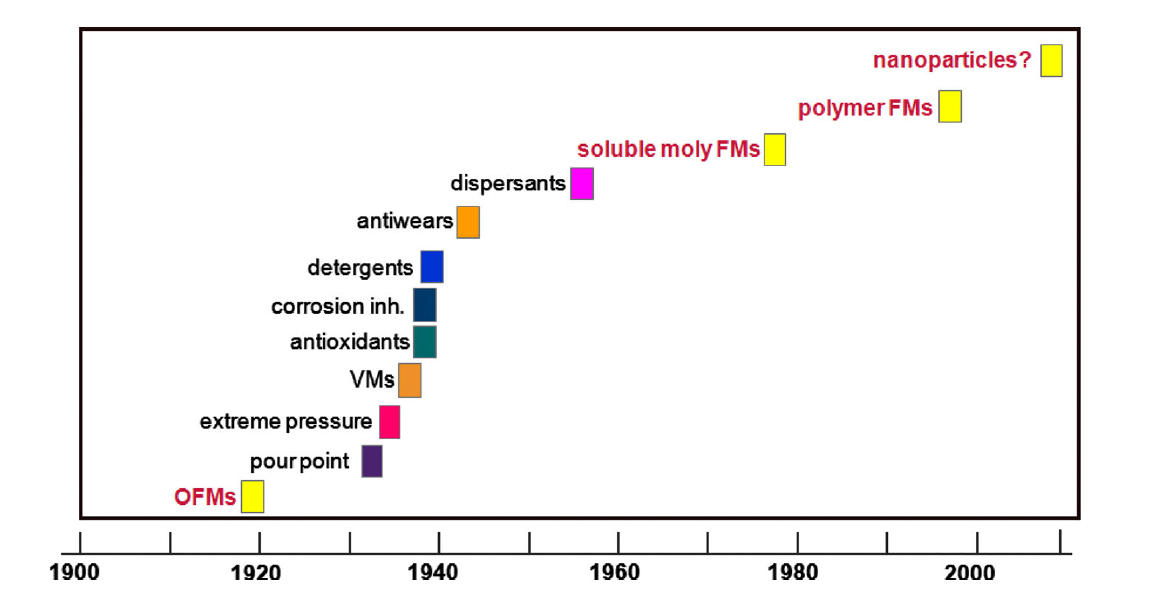
\includegraphics[width=1.0\textwidth]{Chapter-1/fig1_spikes_timeline}
	\caption{Overview of lubricant additives and friction modifiers. Borrowed from Spikes, 2015}
	\label{fig1-spikes-timeline}
\end{figure}


The impetus to change directions from hydrocarbon-based to nanoparticle-based lubricants is not only pushed by the desire to improve human, animal, and environmental health but also pulled by the promise of more effective and efficient lubrication and wear-reduction systems. The impacts of tribology are ubiquitous. Whether discussing economics, the environment, industrial maintenance, changing a car's engine oil, or ice skating,  friction, dissipation, and wear are always issues to be considered. Since the publication of The Jost Report in 1966, interest in and funding for tribological research has accelerated \cite{101}. An oft cited, and important touchstone for the practical importance of tribology, is that a an internal combustion engine utilizing diesel fuel will use 10 \% of the energy from that fuel to overcome internal frictional losses[ZL ref 2,3]. A lowering of those losses to 9 \% is estimated to potentially save one billion gallons of diesel fuel, per year, in the United States. Beyond the fuel expense and diesel exhaust savings, that reduction in frictional dissipation also translates to less wear and tear on the individual engines and thus a potential decrease in maintenance downtime for owners and operators. From this single example, it becomes clear the sort of impacts which tribology is capable of making across the spectrum of the economic and environmental landscapes.


\subsection{Topic 1: Comparison Study of Nanodiamonds Having Positively or Negatively Charged Surface Functional Groups and their Impact on Tribological Behavior}

\subsubsection{Topic 1 Hypothesis}

Following work done by Zijian Liu [cite RSC Adv paper], the predominant hypothesis was that the surface conductivity of a QCM sample would determine which (and whether) a nanodiamond having a particular surface charge, as a function of its surface chemical groups, would experience tribological interactions. It was supposed that an insulating material (Al2O3) and contacting nanodiamond solution would not exhibit significant attraction whereas a conducting material (stainless steel) would exhibit significant attraction, as understood by surface image charge effects.


\subsubsection{Topic 1 Background}

Though the petroleum and synthetic chemical industries have made profound improvements to lubrication in the 20th and early 21st centuries, the secondary effects of these lubricants[insert ref, harmful effects of lubricants] provide strong reason to find novel, less toxic, and more durable lubricants and lubricant additives for both industry, research, and household use. Nanometer-scale particles of many species are emerging as effective lubricant additives [insert ref], much of the work done in oil-based media. Studies of nanodiamonds have shown their ability to lubricate for a long duration with degradation, a common problem for lubricants, though minimal work has been done to examine the lubricant behavior of nanodiamonds in aqueous solution. Further, the importance of surface chemical groups for tribology has been investigated [insert ref]. Here we report the first analysis of the importance to tribology of variation of surface functional groups on nanodiamonds. Carboxylated nanodiamonds were shown to be an effective lubricant for both alumina-on-alumina interfaces as well as stainless-steel-on-stainless-steel interfaces, as tested in a ball-on-disc MTM. On the other hand, hydroxylated nanodiamonds were shown to be either ineffectual in changing the tribology at the interface, for alumina MTM contacts, or to be anti-lubricating, producing an increase in the coefficient of kinetic friction for stainless steel MTM contacts.


\subsection{Topic 2 - The Impact of Root-mean-square (RMS) Surface Roughness on Nanotribological Behaviors for Gold Surfaces}


\subsubsection{Topic 2 Hypothesis}

The study of smooth versus rough gold was conducted following from the hypothesis that a dramatic difference in orders of magnitude difference in the RMS surface roughness of two otherwise identical substrates would have a defining impact on how a set of nanoparticles would interact with those substrates. 

It was proposed that surface geometry at the nanoscale must be known to understand macroscale friction effects.  Nanodiamonds of diameter ~5 nm have a known friction reduction effect (REF 1 - Ozawa, 2007; REF 2 - Liu, 2015,). This effect is thought to be due to polishing of the solution-contacting interface. If the primary action of the nanodiamonds is to polish, there are two possible pathways. It may be that there is a removal of jutting-out asperities OR that there is a filling-in of voids between asperities. The following methods will explore what is occurring at the important scale.

The expectation  at the outset was that a much rougher surface would exhibit a much greater degree of polishing when exposed to a hard particle such as a nanodiamond. If polishing occurs, and the hypothesis is true, this effect ought to be displayed dramatically by gold surfaces having orders-of-magnitude difference in RMS surface rougness between them, as our samples do.



\subsubsection{Topic 2 Background}

This study explores the nanoscale and macroscale tribological attributes of alumina and stainless steel surfaces immersed in aqueous suspensions of positively (hydroxylated) or negatively (carboxylated) charged nanodiamonds (ND). Following on previous work by Dr. Zijian Liu, a Krim group alumnus, this study explores the connection between microscopic (QCM and AFM) effects which result from exposure of metallic and ceramic surfaces to aqueous nanodiamond solutions with the macro-scale lubrication behavior of these same combinations of surfaces and solutions.


\subsection{Topic 3 - The Tribological Behavior of Super-paramagnetic Nanoparticles in Solution at the Interface With and Without the Presence of an External Magnetic Field}


\subsubsection{Topic 3 Hypothesis}

This study explored whether an external, applied magnetic field can influence friction and wear dynamics, at an interface, in the presence of superparamagnetic iron (III) oxide nanoparticles. Such particles have been demonstrated to greatly reduce the volume of material wear when the diameter of the particles was small enough (~30 nm). This reduction in wear is attributed to tribo-sintering of the nanoparticles into a tribo-film on the contacting surfaces (REF 3 and 5  - Kato, 2003, 2008; REF 4 – Kato and Komai, 2006). The production of such a tribo-film is dependent upon the oxygen diffusivity rate of the oxide nanoparticle introduced. High diffusivity among certain oxide species, such as Fe2O3 and Bi2O3, demonstrates a greater ability to produce a tribo-film and in turn dramatically reduce wear volume. This study asks the question: what level of  influence does an external magnetic field exhibit on tribo-film formation, friction, and wear at an interface containing ferrimagnetic nanoparticles, which are otherwise known to lubricate?


\subsubsection{Topic 3 Background}

Certain nanoparticles, gamma-type iron oxide of nominal diameter of 5 nanometers, in this study, exhibit superparamagnetism. Superparamagnetism is the character of a particle such that its entire structure constitutes a single magnetic domain. Thus, as the magnetic moment of the particle respods to an external, applied magnetic field, so does the physical geometry of that particle in terms of its position and orientation. [citations needed]

Previous studies in the NCSU nano-tribology group, conducted by Dr. Zachary Fredricks, explored the paramagnetic behavior of oxygen molecules, at low temperature, in vacuum, on a metallic surface. Through the application and removal of an external magnetic field, the rotational and spatial orientation of these molecules was seen to change, producing an effect in the dissipation as measured by the QCM. [zach thesis citations needed]

The study of superparamagnetic, aqueous iron oxide nanoparticles explores if and how such behaviors manifest in a aqueous, room temperature rather than evacuated, low temperature environment.


\subsection{Topic 4 - Permeation of Gaseous Water and Ethanol into or through Hydrogenated Graphene and Hydrogenated Graphene Oxide}

\subsubsection{Topic 4 Background}
Filtration and Purification, as well as gas separation and retention [ref about helium shortage needed] are practical drivers behind the growing interest in graphene and modified graphene membranes. The study of graphene as a membrane gained particular notoriety upon the observation that a helium-leak-tight graphene membrane is permeable to water\cite{108}. Not only permeable, graphene exhibited extremely low frictional interactions to the diffusion of water through its structure. This work built upon previous work conducted in the Krim Group by Zijian Liu. Whereas his studies utilized graphene membrane layers on top of flat aluminum substrates, the experiments discussed here transition the studies to hydrogenated graphene layers atop nano-porous aluminum oxide substrates. These nano-porous structures, having greater than a billion pores  on the surface of the QCM, increase the working surface area underneath the graphene layers by a factor greater than 100. This great leap in surface area for adsorption of gases which have permeated through the hydrogenated graphene membrane, provide an improvement in sensitivity and reduction of uncertainty in measurements. The porous alumina samples, grown by Dr. Antonin Marek in the NCSU Department of Chemistry, as part of our collaboration with the Smirnov group, follow from well-established methods for anodizing aluminum\cite{109}.

These studies, introducing ethanol and water vapor, separately and during different trials, to the hydrogenated graphene membranes, investigate whether such membranes impede or admit either gas species or if instead the gas species physically or chemically alter said membranes. This work also builds upon work done by Zijian Liu in pursuit of his doctoral degree.

Previous studies, including work done by Nair et al \cite{108}, report the behavior of graphene oxide layers including the impermeability to helium and ethanol. On the other hand, it has been shown that water will flow through a graphene oxide flake layer structure with very low friction. Efforts by Zijian Liu and myself in recording gaseous adsorption isotherms of either water or ethanol demonstrate the behavior of a hydrogenated graphene oxide layer structure in terms of permeability or impediment to flow.

\subsubsection{Topic 4 Hypothesis}


The studies of hydrogenated graphene oxide and hydrogenated graphene layers, on porous alumina substrates, and the exposure of these membranes to either water vapor or ethanol, in vacuum, were conducted following work done in Krim Nanotribology lab[cite Zijian thesis, others], as well as elsewhere in the tribology community[cite Nair et al, others], which demonstrated the impermeability or permeability of graphene and graphene-oxide type membranes to various gaseous species.

Due to the hydrogenation of these two membrane types, graphene and graphene oxide layers, the hydrophobicity of each material was increased [cite C]. The water vapor permeability of each membrane was thus expected to decrease without substantial change in the permeability to ethanol vapor, a non-polar molecule. Comparison with work done by Zijian Liu utilizing un-hydrogenated graphene and graphene oxide layers  is reported.

\addcontentsline{toc}{section}{{Chapter 1 References}}

\printbibliography[title=Chapter 1 References, keyword=one]
\chapter{Experimental Apparatus, Techniques, and Theories of Operation}

\label{chap-two}

In this chapter, the discussion focuses on the experimental devices utilized to conduct experiments and record data for the studies discussed in later chapters. The Atomic Force Microscope (AFM), Scanning Electron Microscope (SEM) and Macro-scale Tribometer (MTM) each play a role. The principal instrument for the work described in this thesis will be the Quartz Crystal Microbalance (QCM) as implemented for both liquid immersion and vapor phase exposure.

\section{Quartz Crystal Microbalance (QCM)}

\subsection{General Description}

 Consisting of conducting electrodes deposited onto thin (<1mm), circular pieces of crystalline silicon dioxide, the QCM is a robust piezoelectric device utilized for nanometer and atomic-scale tribology work \cite{21,22}. Beyond its long-term robust usage as a reliable and robust mass censor elsewhere. Figures 3.1 and 3.2, reproduced from the Dissertation of Dr. Tonya Coffey, displays a QCM as typically used in Krim Lab

\begin{figure}[hbtp]
	\centering
	\includegraphics[width=0.6\textwidth]{Chapter-2/fig1_QCM}
	\caption{QCM Schematic. The QCM is a thin quartz disk. Metal electrodes are	present on both sides of the disk in a keyhole design. Spring clips secure the QCM to the holder and provide electrical contact to the metal electrodes. Leads are attached to	the spring clips. An alternating voltage is applied to the leads that causes our QCM’s	to oscillate. (CITE COFFEY THESIS)}
	\label{fig1:QCM fig 1}
\end{figure}

\begin{figure}[hbtp]
	\centering
	\includegraphics[width=1.0\textwidth]{Chapter-2/fig2_QCM_side}
	\caption{Side view of QCM when it is oscillating in tranverse shear mode. The applied alternating voltage causes the faces of the QCM to move laterally in opposing directions. (CITE COFFEY THESIS)}
	\label{fig2:QCM fig 2}
\end{figure}




The QCM sensors utilized, for the work described hereafter, are of the AT-cut variety with a fundamental frequency of 5 MHz, diameter one inch, and thickness approximately four-tenths of an inch. Utilizing the piezoelectric effect, an oscillating voltage frequency-matched to the fundamental mode of the QCM being used, the QCM oscillates in a shear-transverse mode as depicted in figure 3.2. In vacuum, the quality factor (Q) of these devices, when not inundated by a gaseous species, resides on the order of $10^{5}$. 

Although our lab primarily uses so-called AT-cut QCMs, which given a voltage normal to their flat-surface produce a shear-mode oscillation, other modes are attainable my alteration of the bulk geometry of the crystal. 

\begin{equation}
Q \propto \frac{Energy Supplied}{Energy Lost} \leftarrow per  cycle
\label{ch2-eq:one}
\end{equation}


\subsection{The AT-cut Quartz Crystal}

The AT-cut Quartz Crystal, first mentioned in a 1934 Bell System Technical Journal \cite{211}, provides parts-per-million frequency stability within the temperature ranges considered during this work. The X-cut and Y-cut crystal, the latter of which is displayed in figure 3, represented the integral oscillators for most radio circuitry until the 1930s. 

\begin{figure}[hbtp]
	\centering
	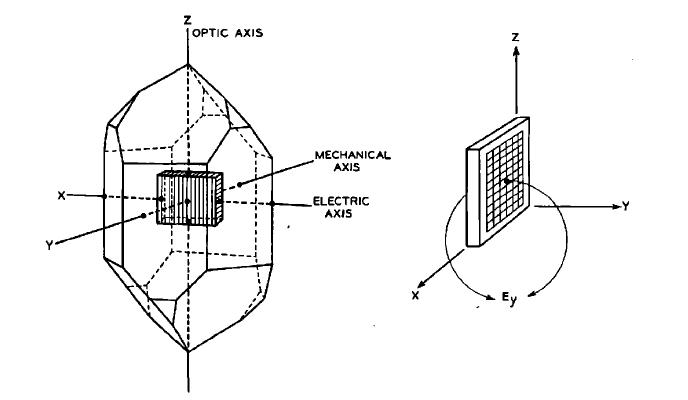
\includegraphics[width=1.0\textwidth]{Chapter-2/fig3_Y_cut_crystal}
	\caption{Representation of how the Y-cut crystal is sectioned from a larger quartz crystal sample. Additionally, the direction of electric field application, for oscillator use, is shown.\cite{211}}
	\label{fig3:Y cut crystal}
\end{figure}





Looking to improve the stability of their their oscillators, researchers at Bell Systems explored the effects of rotating the cut of the crystal by a rotation about the crystallographic x-axis of 31 degrees. This change resulted in drastically improved frequency stability of the resultant oscillator without a proportional loss of piezo-electric activity, as shown in figure 4.


\begin{figure}[hbtp]
	\centering
	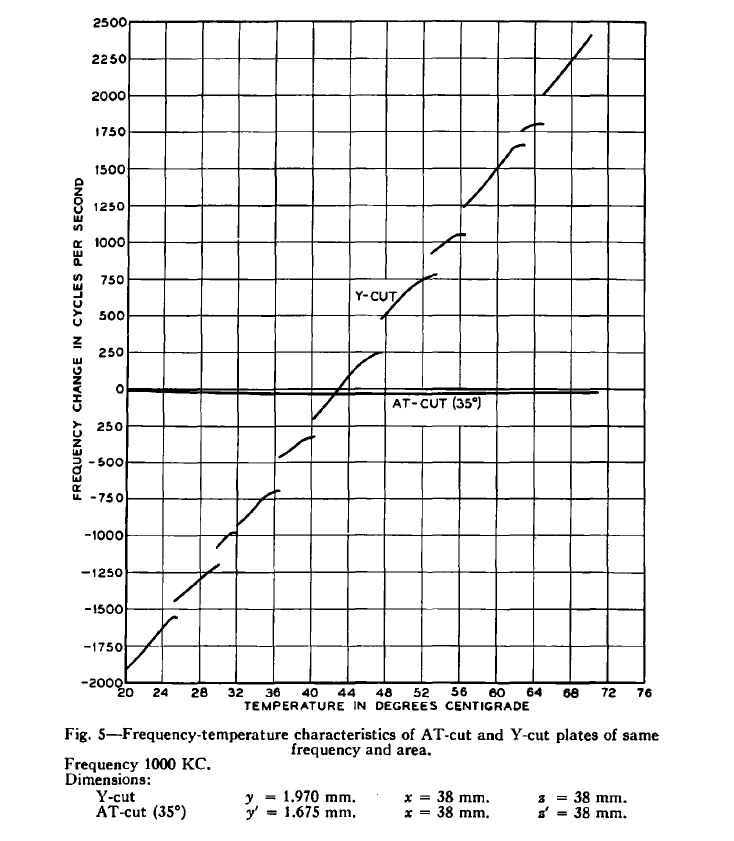
\includegraphics[width=1.0\textwidth]{Chapter-2/fig4_df_vs_T_for_AT_and_Y_cuts}
	\caption{Shift in baseline frequency as a function of temperature for Y-cut and AT-cut crystals, for which temperature stability is improved.\cite{211}}
	\label{fig4:df vs T}
\end{figure}



\subsection{Frequency Shift - Measured}



The crystal oscillators have a stable equilibrium operation mode in both vacuum and aqueous media. In our laboratory tests a frequency drift of less than 1 Hz per hour in aqueous media and performance better than 0.5 Hz per hour in vacuum is typical. For these reasons, the sensitivity to changes in mass at the QCM interface is of great scientific value. While frequency shifts are largely a result of mass-loading, it is critical understand other influences on an observed shift in the QCM frequency during an experiment.



\subsubsection{Mass-loading}

Investigation of rigid-mass-loading on the surface of the QCM was pioneered by M. Sauerbrey, then living in Germany, 1959. Sauerbrey treated adsorbed mass as a small addition to the thickness of the AT-cut (transverse or shear mode) QCM oscillator. \cite{26,27}]

Consider the acoustic, shear-mode oscillation, having speed $\mathit{c_{q}}$ which propagates through the crystal as a product of an applied voltage. The speed of this wave may be decomposed into its wavelength, $\lambda_{q}$ and frequency, $\mathit{f_{q}}$:
	
\begin{equation}
\mathit{c_{q}} = \lambda_{q} \mathit{f_{q}}
\end{equation}
 
Given a crystal fabricated to have a thickness equal to one-half the wavelength of the wavelength above:

\begin{equation}
\mathit{t_{q}} =  \frac{1}{2} \lambda_{q}
\end{equation}

When a film of material is deposited on the surface, the thickness of the oscillator is increased. As can be seen from equations 2.2 and 2.3 above, an increase in oscillator thickness allows an increase in the wavelength, $\lambda_{q}^{'}$ and a decrease in the frequency, $\mathit{f_{q}^{'}}$. The speed of the acoustic wave is assumed to remain constant in the crystal.

\begin{equation}
\mathit{c_{q}} = \lambda_{q}^{'} \mathit{f_{q}^{'}}
\end{equation}

If we take the new film on the surface of the oscillator, having thickness $\mathit{t_{film}}$, and add it to the thickness of the quartz oscillator, $\mathit{t_{q}}$ and recalling that we work from the assumption that the film is rigidly attached to the oscillator's surface, we may right the new thickness of the oscillator $\mathit{t^{'}}$ as:

\begin{equation}
\mathit{t'}= \mathit{t_{film}} + \mathit{t_{q}}
\end{equation}

Bringing in the rigidly-attached film's mass, $\mathit{m_{film}}$, surface area $A$, and with the film's thickness previously defined as $\mathit{t_{film}}$, we may then write the mass density, $\rho_{film}$, of the film as

\begin{equation}
\rho_{film} =  \frac{m_{film}}{A t_{film}}
\end{equation}

Solving equation 2.2 for $\lambda$ and combining it with equation 2.3 produces

\begin{equation}
\mathit{f_{o}} = \frac{c_{q}}{2t_{q}}
\end{equation}

Our interest is in how the frequency changes as a function of the addition of an adsorbed film, so we might differentiate the frequency $f$ in equation 3.6 with respect to the changing thickness of the system, $t'$

\begin{equation}
\frac{\mathrm{d}f_{q} }{\mathrm{d} t_{q}} = \frac{\mathrm{d} }{\mathrm{d}t_{q}}\frac{c_{q}}{2t_{q}}
\end{equation}

Examining equations 2.7 and 2.8 closely for which terms might be cancelled out by operating one on the other, a maneuver appears. Dividing equation 2.7 by equation 2.8 produces

\begin{equation}
\frac{\mathrm{d}f_{q}}{f_{q}} = \frac{-\mathrm{d}t_{q}}{t_{q}}
\end{equation}

Taking a brief detour backwards, re-arrange equation 2.6 to solve for the film's mass, $\mathit{m_{film}}$
\begin{equation}
\mathit{m_{film}} = \rho_{film}A t_{film}
\end{equation}

Our interest is in how a small change of the frequency of the oscillator, a directly measurable quantity, can be utilized to learn the change in mass on the QCM surface in the form of that added film thickness.

\begin{equation}
\Delta \mathit{m_{film}} = \rho_{film}A \Delta t_{film}
\end{equation}

Saurbrey's idea was that if a film were to be considered to be rigidly attached to the surface of the oscillator, then the layer of added material under consideration should be approaching the infintesimal, and so equation 2.11 moves towards that limit to produce


\begin{equation}
d\mathit{m_{film}} = \rho_{film}A dt_{film}
\end{equation}

Equation 2.9, which describes the relative, infinitesimal change in frequency associated the relative, infinitesimal change in the crystal's thickness now seems an appropriate place to substitute in equation 2.12 after it has been solved for change in film thickness, $dt_{film}$

\begin{equation}
\frac{\mathrm{d}f_{q}}{f_{q}} = \frac{-\mathrm{d}m_{film}}{t_{q}\rho_{film}A}
\end{equation}

Recall that we are principally interested, with this treatment, in loading the QCM with a mass such that $dm_{film} << m_{q}$. Defining the speed of the sheer oscillation as $v_{q} = \frac{f_{q}}{\lambda_{q}}$, the widely-reknowned Saurbrey Equation for one-sided film-growth is written
\begin{equation}
\Delta f = \frac{-\Delta m_{film}f_{q}^{2}}{A\rho_{film}v_{q}}
\end{equation}

The above relationship may be used to convert a measured shift in the resonant frequency of the QCM to a value for mass added to the interface of the QCM if the adhered film:

\begin{enumerate}
	\item covers the portion of the QCM which is in motion uniformly
	\item is non-dissipative (no slip OR slip with zero friction?)
	\item has a mass which is much smaller than the mass of the oscillator as a whole
	\item is rigidly attached to the surface
\end{enumerate}

The Saurbrey equation, and his reasoning, are a special case for the interaction of an adsorbed film on the surface of an oscillating quartz crystal microbalance. Despite several decades of use since his work, and more general approaches being developed, the Saurbrey equation remains a gold standard for nanotribology. Mass-loading is responsibile for the greatest portion of frequency shifts observed for the work reported in this thesis.









\subsection{Energy Dissipation at the QCM Interface}

\subsubsection{Amplitude - Measured}

Amplitude of oscillation, in volts, is the other quantity measured from a QCM in operation.  Generally speaking, as the amount of energy lost at the interface between the QCM surface and its counter-face increases, the amplitude will decrease. This is not a complete picture as the QCM-oscillator-system may also lose energy internally.


\subsubsection{Quality Factor}

The quality factor, $Q$, describes the degree of damping in an oscillating system. The QCM system is an electrical circuit driving a physical oscillator, both of which feedback into the other. Provided that the electronics are well-insulated from disturbance, the a shift in Q, for the QCM system, indicates and increase or decrease in energy dissipation at the interface. A useful,  definition for $Q$ is given as follows in equation 2.15:

\begin{equation}
Q = 2* \Pi* \frac{Energy Added per Cycle}{Energy Lost per Cycle}
\end{equation}

Electrical energy is added to the system by driving circuitry while dissipation of energy occurs either through inter-facial or internal mechanisms. Inversely proportional to the quality factor is then readily defined as the dissipation factor, $D \alpha Q^{-1}$

\subsection{Slippage at the QCM Interface}

Slippage, or phase delay, between materials and the QCM surface itself results in dissipation of energy. The effect of a film moving out-of-phase with the QCM, ie slipping, has been calculated by Bruschi and Mistura. (L Bruschi and G. Mistura, Phys Rev B 63, 235411 2011).

This slippage at the interface adds a component to the impedance of the system. This is critical for a full treatment of few-molecule adsorbtion to the QCM in vacuum. Additionally, it provides insight into the mechanism by which the QCM in liquid loses energy with each cycle. This additonal impedance is defined as $\frac{1}{\eta_{2}}$.

\subsection{The Behavior of the QCM, in Vacuum, in the Presence of Gaseous Species - Adsorption Isotherms}



\subsection{The Behavior of the QCM in Liquid Environments}

\subsubsection{Temperature}

Use of AT-cut quartz crystals

\subsubsection{Pressure}

\begin{figure}[hbtp]
	\centering
	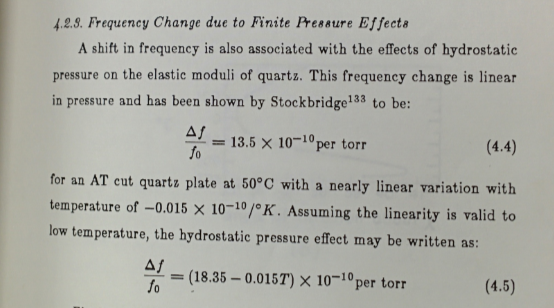
\includegraphics[width=1.0\textwidth]{Chapter-2/fig3_krim_thesis_QCM_pressure_effect}
	\caption{THIS IS A PLACEHOLDER - needs to be swapped for specifics refs to Krim Thesis (1984) and Stockbrige, Ref 133 from that thesis}
	\label{fig5:QCM_pressure}
\end{figure}



\subsubsection{Stress -and changes in pressure?-}

\section{LabVIEW Recording Software for QCM Experiments}


\section{The Atomic Force Microscope}

Observations of surface roughness for materials, before and after their exposure to tribological processes, provides information regarding etching, polishing, or other wear behaviors. The AFM was the principle tool used in this work to characterize material surfaces for these purposes. The principles of operation of the AFM apparatus generally, as well as pertinent speficics of the platform used to take the measurements described in this work, are as follows.



\section{Scanning Electron Microscope}




\section{Vacuum Systems}









\section{Equipment for Liquid-immersed QCM Measurements}



\subsection{Stanford Research Systems Flow Cell}



\subsubsection{Flow Cell Electronics}




\section{Macro-scale Friction Measurements}



\subsection{Background and Conventions for Macro-scale Tribology}

Testing for wear, friction, and lubrication between macro-scale contacts is of obvious importance for nearly any industrial or commercial enterprise which uses stationary machinery or transportation equipment. In the research setting, a macro-scale tribometer is useful as a means of testing novel lubricants or additives. The observations from such macro-scale tests, which are often cheaper, easier, and faster to conduct than many fine or even atomic scale measurements, can contribute to a tighter feedback loop in tribological studies. Critically, employment of a macroscale tribometer allows for correlation between lubrication and wear in practical settings with the behavior of nanoparticles at the interface as observed with other research implements.


\subsection{PCS Instruments MTM-2 Macro-scale Tribometer}



\section{Dynamic Light Scattering and Electrophoresis Measurements for Nanometer Size Particle Characterization}





\subsubsection{Principles of Dynamic Light Scattering}



\subsubsection{Principles of Electrophoresis}

For any set of nanoparticles in aqueous solution, it is necessary that they exhibit a mutual electro-static repulsion lest they agglomerate with one another, changing physical, optical, and other properties of critical interest. The mechanism by which aqueously suspended particles maintain their distance is electro-static repulsion(CITATION NEEDED). Typically characterized by a zeta potential, $\zeta$, measured in millivolts, the degree of repulsion is determined through use of an electrophoresis measurement (CITATION NEEDED).

By applying an electric field across a sufficiently dilute sample, particles within the sample will begin to move parallel to the direction of the field. The speed at which the particles move, on average, is a function of the field strength as well as the net charge, $Q$, on the constituent particles. The force experienced by each particle may be written as follows.

\begin{equation}
\mathit{f} = E \times Q
\end{equation}



The velocity is determined by means of a doppler-shift in a LASER signal directed into the liquid sample.

\subsubsection{Malvern ZetaSizer Specifics}








\addcontentsline{toc}{section}{{Chapter 2 References}}
\printbibliography[title=Chapter 2 References, keyword=two]
\chapter{Theory and Fundamentals - Nanostructured Materials, Charge, Zeta Potential, Aqueous Kinetics}

\label{chap-three}

\section{Nano-porous Alumina}

Experiments conducted on a QCM surface benefit from an increase of surface area. As the surface area increases, in general the amount of mass adsorbed and energy dissipated, all other environmental and material factors being equal, will increase. In effect, increasing the surface area acts as a gain. To that end, many aluminum samples in this work have been anodized unto the formation of pores.(cite Toborek, etc)

In an Oxalic acid bath, the Aluminum-coated QCM is the cathode.  Applying a voltage to the system, charges on the surface of the cathode self-organize in a hexagonal close-packed pattern and begin the oxidation process, boring into the aluminum substrate.




\subsection{Electronic Surface Structure of Alumina}

\subsection{Geometry of Nano-porous Alumina and Effects on Phase Transitions}





\section{Graphene Membranes}

\subsection{Electronic Surface Structure of Nanodiamonds}






\section{Graphene Oxide Membranes}

\subsection{Electronic Surface Structure of Nanodiamonds}







\section{Nanodiamonds}

\subsection{Detonation Nanodiamond Synthesis}



\subsection{Molecular Adsorption and Bonding of Functional Groups to Nanodiamond Surfaces}

\subsubsection{Electronic Surface Structure of Nanodiamonds}



\subsection{Functional Groups, Surface Charge, and Zeta Potential}



\subsection{Aqueous Kinetics of Nanodiamonds}



\addcontentsline{toc}{section}{{Chapter 3 References}}

\printbibliography[title=Chapter 3 References, keyword=three]
\chapter{Sample Preparation}
\label{chap-four}

\section{QCM Sample Preparation and Details}

\subsection{Crystal Growth and Preparation}

\subsection{QCM Electrode: Material Choice, Suppliers, and Deposition Techniques}

\subsubsection{Stainless Steel, Aluminum, Gold - Filtech}

\subsubsection{Graphene and Graphene Oxide Preparations - NRL}


\section{De-ionized Water Source and Details}

\section{Nanoparticles}

\subsection{Nanoparticle Synthesis}

\subsection{Nanoparticle Surface Modification and Characteristics}

\section{List of Samples Used in Experiments, by Type}

\subsection{Quartz Crystal Microbalances and Affixed Materials}

\subsection{Nanoparticle Solutions}

\subsection{Adsorbate Species for Adsorption Isotherm Work}

\subsection{Macroscale Tribometer Samples}


 




\addcontentsline{toc}{section}{{Chapter 4 References}}
\printbibliography[title=Chapter 4 References, keyword=four]
\chapter{A Comparative Study of The Nanoscale and Macroscale Tribological Attributes of Alumina and Stainless Steel Surfaces Immersed in Aqueous Suspensions of Positively or Negatively Charged Nanodiamonds (reprint)}
\label{chap-five}

Colin K. Curtis1, Antonin Marek2, Alex I. Smirnov2 and Jacqueline Krim*1

\section{Abstract}

This article reports a comparative study of the nanoscale and macroscale tribological attributes of alumina and stainless steel surfaces immersed in aqueous suspensions of positively (hydroxylated) or negatively (carboxylated) charged nanodiamonds (ND). Immersion in −ND suspensions resulted in a decrease in the macroscopic friction coefficients to values in the range 0.05–0.1 for both stainless steel and alumina, while +ND suspensions yielded an increase in friction for stainless steel contacts but little to no increase for alumina contacts. Quartz crystal microbalance (QCM), atomic force microscopy (AFM) and scanning electron microscopy (SEM) measurements were employed to assess nanoparticle uptake, surface polishing, and resistance to solid–liquid interfacial shear motion. The QCM studies revealed abrupt changes to the surfaces of both alumina and stainless steel upon injection of –ND into the surrounding water environment that are consistent with strong attachment of NDs and/or chemical changes to the surfaces. AFM images of the surfaces indicated slight increases in the surface roughness upon an exposure to both +ND and −ND suspensions. A suggested mechanism for these observations is that carboxylated −NDs from aqueous suspensions are forming robust lubricious deposits on stainless and alumina surfaces that enable gliding of the surfaces through the −ND suspensions with relatively low resistance to shear. In contrast, +ND suspensions are failing to improve tribological performance for either of the surfaces and may have abraded existing protective boundary layers in the case of stainless steel contacts. This study therefore reveals atomic scale details associated with systems that exhibit starkly different macroscale tribological properties, enabling future efforts to predict and design complex lubricant interfaces.

\section{Introduction}


Interest in nanoparticles as eco-friendly lubricant additives has grown tremendously in recent years [4.1,4.2]. The field is driven in a large part by a pressing need to replace hazardous additive materials in present-day oil-based lubrication technologies and to eliminate the serious environmental risks associated with oil leakage and disposal [4.3-5]. Water-based lubricant systems are a particularly attractive target for nanoparticulate additives since conventional oil additives generally fail to improve tribological performance in aqueous environments. Numerous studies of nanoparticulate additives to oil-based systems have been reported in the literature, with many displaying significant improvements in macroscopic friction and wear rates [4.6]. Water-based suspensions have received far less attention [4.1,2,79]. Although the low shear strength of water is beneficial in the hydrodynamic regime of lubrication, under normal loads it also enables contact between opposing surfaces. Nanoparticulate additives have the potential to overcome this deficiency, by penetrating into contacts where they may form boundary films and/ or act as rolling or sliding spacers (Figure 1) [4.6,10,11]. As such, nanoparticles exhibit a great potential for replacement of the centuries-old oil-based lubricating technologies.

Tribological studies of water-based nanoparticle suspensions reported to date have mostly involved NDs. Reductions in kinetic friction coefficients µk by factors of 5–20 have been reported for metallic [4.7], ceramic [4.8], and semiconducting materials [4.2]. It is likely that the literature is reporting primarily on those nanoparticle additives with a beneficial tribological performance. 

\begin{figure}[hbtp]
	\centering
	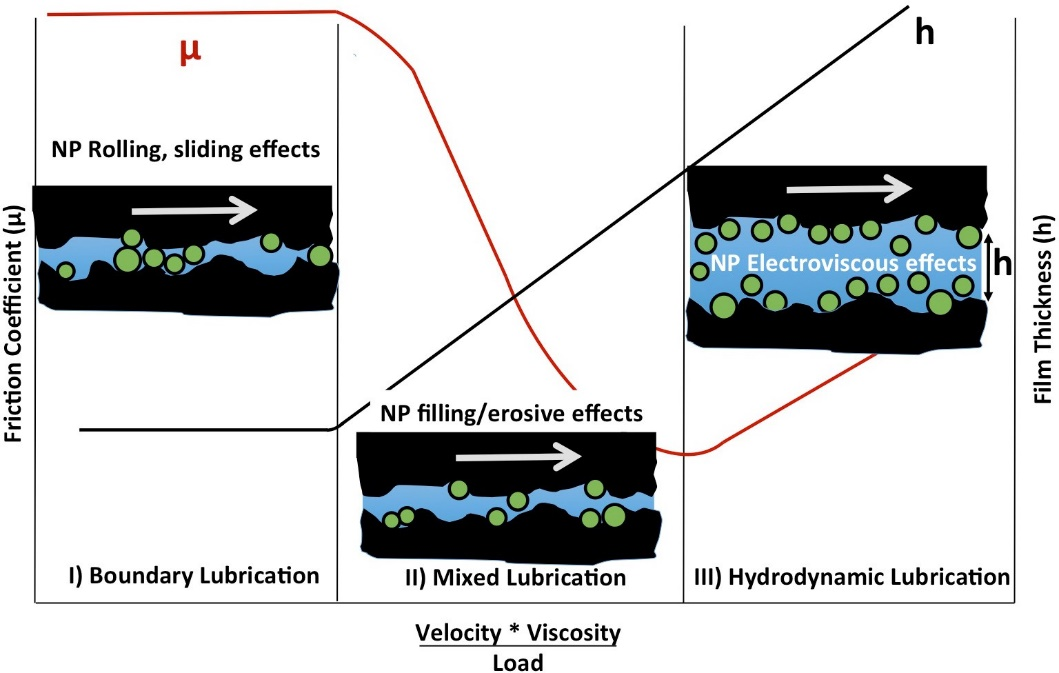
\includegraphics[width=1.0\textwidth]{Chapter-4/fig1_png}
	\caption{Friction coefficient plotted as a function of fluid viscosity and shear velocity divided by load (Stribeck curve). NPs present in a fluid could impact the tribological performance in all three lubrication regimes, for example by forming lubricious surface coatings or acting as rolling or sliding spacers at the contacts. In addition they may potentially fill or erode the contacts and/or cause the solid–fluid interfacial slip attributes to change via electroviscous and/or steric mechanisms. See text for further discussion.}
	\label{fig1: 3 lub regimes}
\end{figure} 

Identification of nanoparticulate additives that are detrimental and/or have no effect have received much less attention even though such data are exceptionally useful for the purposes of evaluating test models [4.12]. Liu et al. recently investigated the tribological performance of steel/gold contacts in water using both nano- and macroscale measurements and found the contact to be highly sensitive to the sign of the charge on the NDs in suspension [4.9]. The authors suggested that the −ND suspensions were more likely to improve the tribological performance in macroscale settings than the +ND suspensions, and speculated that the electrostatic properties of the materials in contact might play a role. Generally, NDs require surface chemical treatments in order to be electrically charged in aqueous suspensions so as to inhibit aggregation via a mutual electrostatic repulsion, similar to other nanoparticles [4.2,9,13-15]. These chemical treatments are well known, however, to impact the friction coefficients in humid and dry environments for standard tip on disk geometries [4.16,17]. The surface chemical treatments employed in the production of the ND might therefore dominate the tribological performance. The surface charges on ND are also expected to affect the interfacial solid–fluid slip lengths attributes, and therefore the apparent fluid viscosity, via electroviscous and/or steric mechanisms [4.18-20]. Fundamental studies at the nanoscale are clearly essential at this time in order for the field to progress and for accurate model predictions to be developed.
QCM is emerging as an ideal tool for studying the fundamental mechanisms associated with nanoparticle lubrication [4.9]. While historically it was developed as a time standard and a deposition rate monitor for thin films [4.21], it has rapidly expanded in recent years to a broad range of applications through simultaneously monitoring of changes in frequency and quality factors [4.22-26]. It has become well known as a nanotribological technique for studying uptake and sliding friction levels of films in both in vacuum and liquid environments [4.23-25]. When immersed in liquid, it can be used to probe frictional drag forces and interfacial effects at complex solid–liquid interfaces [4.19,27] including those of a biological origin [4.18,22]. Given that the transverse shear speed of the oscillating QCM electrode is generally in the range of mm/s to m/s [4.23], it can readily be compared to conditions of macroscopic friction measurements. In addition, QCM experiments can be performed using an electrode in a rubbing contact with another macroscopic surface, for example a ball bearing [4.9,26], yielding important information on the shear strength and friction coefficients associated with macroscopic contacts.
For the present study, the QCM technique was employed to perform a comparative analysis of the tribological parameters of aqueous suspensions of either positively (hydroxylated) or negatively charged (carboxylated) NDs for the surfaces with contrasting electrical properties, namely insulating ceramic (alumina) and electrically conducting (stainless steel) surfaces immersed in suspensions of either positively (hydroxylated) or negatively charged (carboxylated) NDs (Figure 2).

\begin{figure}[hbtp]
	\centering
	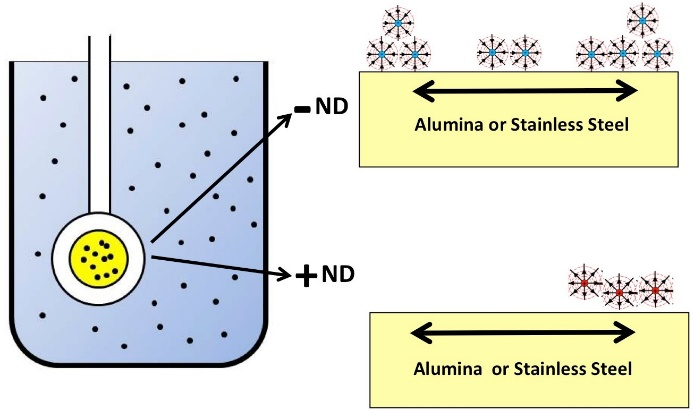
\includegraphics[width=1.0\textwidth]{Chapter-4/fig2_png}
	\caption{Schematic of a QCM immersed in aqueous suspensions of −ND and +ND, for sliding friction studies on materials with contrasting electrical properties, namely alumina and stainless steel. Adapted with permission from [4.9], copyright 2015, Royal Society of Chemistry.}
	\label{fig2: SRS-in-beaker}
\end{figure} 

The QCM measurement experiments were complemented by AFM and SEM measurements of the surface topography before and after the ND exposure, as well as macroscale measurements of µk. The materials were inspired by Liu et al.’s suggestion that differences in the tribological properties between +ND and −ND suspensions might originate in electrostatic effects [4.9], since the electrical charge carriers in the QCM electrodes might respond differently to positively and negatively charged nanoparticles. Would the effect therefore be absent for insulating materials? Was the explanation viable given the symmetry of electrostatic forces?
As will be reported, beneficial tribological behaviors were observed for immersion of stainless steel or alumina samples in −ND suspensions, while either neutral (alumina) or detrimental (stainless steel) behaviors were observed for immersion in +ND suspensions. This yields an exceptional opportunity for crosscomparisons with atomic scale tribological probes. At the atomic scale, the QCM and microscopy studies indicated uptake of particles, along with the potential presence of lubricious slurry for the −ND suspensions, somewhat analogous to boundary lubrication and steric repulsion effects by mucinous glycoproteins boundary layers in aqueous biological settings [4.18]. Such behavior was not observed for the +ND suspensions. The nanoscale mechanisms associated with effective lubrication therefore include boundary film deposits in combination with low interfacial resistance to shear motion in the suspension.

\section{Materials and Methods}

\subsection{Materials}

Aqueous suspensions of 5 nm detonation NDs with oppositely charged zeta potentials were purchased from Adamas Nanotechnologies (Raleigh, NC). All other chemicals were purchased from Sigma-Aldrich (St. Louis, MO) or Acros Organics (Morris Plains, NJ). The −ND samples were carboxylated [4.2,28], (part \# ND5nmNH20) and as manufactured have an average particle size of 5 nm and a zeta potential of −50 mV [4.29]. The +ND samples were hydroxylated in the course of a reduction reaction [4.28], (part \# ND5nmPH20) and, as manufactured, have an average particle size of 5 nm and a zeta potential of +45 mV. The suspensions were employed as received from the manufacturer in the form of 1 wt\% slurries in DI water, and stored without exposure to light. The suspensions were diluted tenfold by volume in advance of experiments using DI water to yield 0.1 wt\% suspensions employed in all measurements. While both stock and the diluted suspensions were found to be stable over a short storage up to 1 month, some slow agglomeration has been observed over a prolonged storage (e.g., see [4.9,29]).

Macroscale friction measurements were performed with ballon-disk contacts of like materials. Alumina (Al2O3) ball and the disk contacts were purchased from PCS Instruments (London, United Kingdom), with respective part \#’s MTMB3/4AL2O3 and MTMD3/4AL2O3.
Stainless steel (AISI 52100) polished ball and the disk contacts were also purchased from PCS Instruments (London, United Kingdom), with respective part \#’s BALLD and MTMPD.
Unpolished 304 stainless steel penny washers (part \# HYWM10-45-A2) were purchased from AccuGroup, (Huddersfield, United Kingdom) (304 stainless steel is also referred to as A2 stainless steel) and were employed as disks for selected measurements. Before the macroscale friction measurements all surfaces were cleaned in ethanol and then DI water.
5 MHz polished QCM crystals (1” diameter) with either stainless steel (SS304; part number QM1022) or aluminium (part number QM1010) electrodes on the liquid facing side were purchased from Fil-Tech (Boston, MA). The QCM’s were specifically designed for operating with one surface immersed in a liquid at a fundamental transverse shear mode. The aluminum QCM samples were anodized using a literature method that grows an alumina layer at the rate of 2 μm/h [4.30]. For these results, the liquid side QCM electrode was connected as the anode and the sample was then immersed into 4 wt\% oxalic acid solution maintained at 0 °C. A cathode was placed in the bath and an electric potential of 40 V was applied between the anode and the cathode. Anodization was halted at 3 min yielding an approximately 100 nm thick Al2O3 layer. After the anodization procedure, the samples were thoroughly rinsed with DI water before mounting the sample within the flow cell.

\subsection{Macro-scale Friction Measurements}

Macroscopic scale friction coefficient measurements were performed with a MTM2 Mini-Traction Machine (PCS Instruments, London, UK). The apparatus is capable of measuring frictional properties of both lubricated and unlubricated contacts under either both sliding and rolling conditions. Its test specimens consist of a 19.05 mm (3/4 inch) ball and a 46 mm diameter disc. The ball is loaded against the face of the disc and the ball and disk are driven independently to create a mixed rolling/ sliding contact. Force transducers measure the frictional forces, and additional sensors are present to measure the loading force and lubricant temperature in real time. For the measurements reported here, the setting were adjusted to a normal load of 4 N with a ball rolling speed of 200 mm/s and a slide to roll ratio of 90\%, which resulted in a smooth friction coefficient versus time signal for both stainless steel and alumina contacts. Lubrication under such conditions allows one to probe of the ability of nano-particulates to penetrate the contacts when they are introduced to fluids surrounding a contact [4.10].
A series of alumina–alumina and stainless steel ball on disk combinations were studied, ranging from pristine as-manufactured samples to samples that had experienced multiple exposures to DI water and ND suspensions. Contacting materials included both the alumina and stainless steel substrates obtained directly from the instrument manufacturer or stainless steel penny washers situated in place of the disk while in contact with the stainless steel ball.

\subsection{Atomic Force Microscopy and Scanning Electron Microscopy Characterization of Surface Topology}

Surface topology characterization of the QCM electrodes was performed with an Asylum Research MFP 3D AFM equipped with silicon nitride tips (part\#NCHV-A, Bruker AFM Probes, Camarillo, CA) and operated in a tapping mode. The 1024 × 1024 images were recorded at a rate of 1 line/s yielding a height profile h = h(xi,yi). The height profiles were quantified by the rms roughness value σ, which is virtually always dependent on the size of the area sampled below a characteristic lateral correlation length ξ. For a self-affine fractal surface the rms roughness increases with the lateral length of the sampled area as σ   LH, where H is the roughness exponent whose value lies between 0 and 1. Fractal surfaces are often characterized by self-affine fractal dimension D = 3 − H [4.31-33]. Self-affine surfaces have an upper horizontal cut-off length (the lateral correlation length (ξ)) above which the rms roughness saturates towards a value of σs and no longer exhibits fractal scaling. The surface roughness parameters (D, ξ and σs) reported herein were obtained from the log(σ) vs log(scan size) plot method as described by Krim and co-workers [4.32]. Previously, a detailed comparison of the results obtained by this method to several literature approaches yielded roughness parameters within experimental error of each other [4.33]).
Scanning electron microscope imaging was performed using an FEI Verios 460L field-emission microscope. A high resolution through-the-lens detector was used in a beam-deceleration mode for ultra-high resolution backscatter imaging of flat samples. For a typical SEM imaging, a whole QCM crystal (1” in diameter) was attached to a pin mount using a small piece of a double sided carbon tape. Sets of images at different magnifications ranging from 5 × 103 to 350 × 103 were recorded under typical settings of an accelerating voltage and a bias of 2.00 kV and 200 V, respectively.

\subsection{Quartz Crystal Micro-balance Apparatus}

QCM data were collected using a QCM 100 (Stanford Research Systems, Sunnyvale, CA, USA) system. The system includes a controller, oscillator electronics and a Teflon holder and a flow cell that exposes one side of the crystal to approximately 0.15 mL of liquid, as well as providing mechanical support and electrical connections to the QCM electrode. All QCM experiments were carried out at room temperature and the temperature was stabilized by the thick, insulating polymer walls of the flow-cell apparatus, as evidenced by the flatness in the frequency during initial and final water exposures. All liquids were kept adjacent to one another on the lab bench during the experiment to minimize temperature differences between them. A LabVIEW (National Instruments, Austin, TX) PC-based data acquisition system was used to record both the crystal resonant frequency and the conductance voltage Vc, from the controller output. The conductance voltage, Vc, is related to the mechanical resistance, Rm, as   [4.34]. Changes in mechanical resistance are directly proportional to changes in the inverse quality factor of the resonator, as will be described below.
Data were recorded as follows. The QCM sample was first placed into the flow-cell initially filled with ambient air. The system was operated continuously until the frequency and amplitude stabilized to less than 1 ppm/min. Once this stabilization occurred, DI water was injected into the flow-cell. Following 1 h water exposure, 10 mL of aqueous 0.1 wt\% ND suspension was flushed into the flow-cell using a syringe pump. The use of a large excess of ND suspension ensured complete replacement of the DI water in the cell. Following 1 h of exposure to the ND suspension, 20 mL of DI water was flushed into the cell by a second syringe pump.

\subsection{Quartz Crystal Micro-balance Data Analysis}

Analogous to the description in [4.9], changes in the resonant frequency, δf , and the inverse quality factor, δ(Q−1), of a QCM reflect changes in the mass and frictional energy losses of materials deposited onto its surface electrodes and/or drag forces and interfacial slippage of fluids that it is immersed in. For a QCM with one side immersed in a fluid with bulk density ρ3 and viscosity η3, the shifts in δf and δ(Q−1) associated with the presence of the liquid under no-slip boundary conditions are given by [4.35]:

\begin{equation}
\delta (Q^{-1})=2\alpha,  \delta = -\mathit{f}\alpha , where\rightarrow \alpha= \sqrt{\frac{\rho_{3}\eta _{3}\mathit{f}}{\pi\rho_{q}\mu _{q}}}\mathit{f}
\label{ch5:eq1}
\end{equation} 

where ρq = 2.648 g/cm3 is the density and µq =
2.947 × 1011 g/cm/s2 is the shear modulus of quartz. Immersion of one side of a 5 MHz resonant frequency QCM in water at room temperature (ρ3 = 1 g/cm3, η3 = 0.01 poise) results in a δf = −714 Hz drop in the resonant frequency and an increase of δ(Q−1) = 2.85 × 10−4 in the dissipation. For a QCM with quality factor Q = 50,000 in air this corresponds to a drop to Q = 3,280 after an immersion in water.
The viscous drag forces on the QCM electrode are mechanical in nature; a decrease in Q is manifested as an increase in the series resonant resistance Rm of the QCM resonator that can be measured electrically. For a QCM electrode exposed to a fluid from one side under non-slip conditions [4.36,37]:

\begin{equation}
\delta (R_{m})=\frac{1}{8\mathit{K^{2}C_{0}}} \sqrt{\frac{\pi\rho_{3}\eta _{3}\mathit{f}}{\mathit{f}\rho_{q}\mu _{q}}}
\label{ch5:eq2}
\end{equation} 

where K2 = 7.74 × 10−3 is the electromechanical coupling factor for the AT cut quartz (AT stands for temperature compensated transverse shear mode type A) and C0 is the static capacitance of the QCM electrodes, including the parasitic capacitance associated with the connections to the oscillator circuit. A comparison of Equation 2 and Equation 3 reveals that δRm is directly proportional to δ(Q−1): Both are reflective of the oscillator dissipative behaviour. For the QCM system employed here, the theoretical value for δRm increase associated with the immersion of a 5 MHz resonant frequency QCM in water is approximately 300 Ω.

In practice, the frequency shifts observed upon immersion into a liquid environment are larger than those predicted by Equation 1 for perfectly planar QCM electrodes. This effect is attributed to the roughness of the surface electrode and can be minimized by using overtone polished crystals, but cannot be completely neglected because no surface has perfectly zero roughness. The magnitude of this contribution has been estimated to be in the range of 2–10\% for materials with rms roughness of the same order as the QCM electrodes employed here [4.36-41]. Therefore, if a QCM surface immersed in a liquid becomes rougher or smoother while immersed in a liquid suspension of nanoparticles, its frequency will drop or increase in unison. A similar response is present also for the changes in the mechanical resistance.

In addition to the aforementioned contributions, nanoparticles may rigidly adhere to the surface when introduced into a liquid, resulting in further changes to the frequency and quality factor of the QCM in association with their mass loading effects. As originally reported by Sauerbrey, an additional rigidly adhering film deposited onto one side of a QCM will decrease its resonant frequency by [4.21]:

\begin{equation}
\delta (f_{film})=-\frac{m_{f}}{A}  \frac{2f^{2}}{\sqrt{\rho_{q}\mu _{q}}} = - 2.264 \times  {10^{-6}}\times  \rho_{2}f^{2}
\label{ch5:eq3}
\end{equation} 

where ρ2 = (mf/A) is the mass per unit area of the film in g/cm2. This equation is the main basis for the use of QCM as a mass sensor in vacuum applications where the Equation 1 contributions from a surrounding fluid are absent. Martin et al. studied the effect of simultaneous mass and liquid loading on QCM and demonstrated that Equation 1 and Equation 3 can be added linearly to obtain the combined effect so long as the mass is not slipping on the surface electrode [4.36]. Therefore the frequency shift associated with mass uptake from a liquid is the same as mass uptake from a vacuum.

\begin{figure}[hbtp]
	\centering
	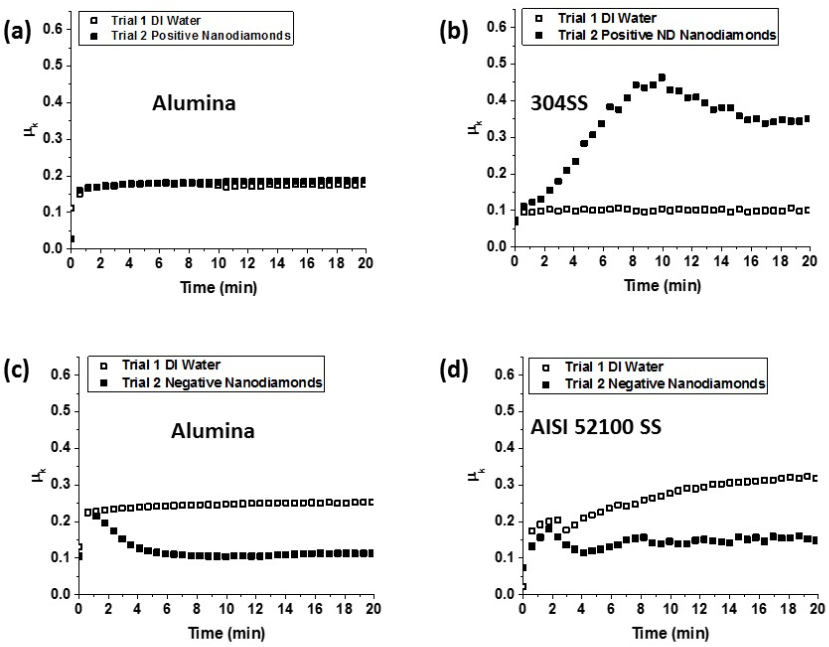
\includegraphics[width=1.0\textwidth]{Chapter-4/fig3_png}
	\caption{Representative friction coefficient versus time plots for alumina (left) and stainless steel (right) contacts lubricated with pure DI water (open squares), positively (a,b) and negatively (c,d) (filled squares) charged ND suspensions. Addition of −ND to water (c,d) consistently lowered the friction coefficient while addition of +ND to water consistently (a,b) failed to lower the friction coefficient.}
	\label{fig3:MTM plots}
\end{figure} 

If the adsorbed particles slip on the QCM surface in a response to the oscillatory motion, and/or the no-slip boundary conditions are altered at the upper boundary of the film with the surrounding liquid, the magnitude of the frequency shift δffilm will be lower than that of a rigidly attached film [4.27,37,40]. These effects may cause the liquid’s effective viscosity to appear to increase or decrease due to electroviscous or steric effects [4.19]. They will also be reflected in the QCM’s quality factor, Q, since the friction associated with the oscillatory motion is manifested in the quality factor. Therefore, while the exact details of the complex solid–liquid–nanoparticle interface may be unknown, changes in the quality factor reflect outright the frictional resistance forces at the interface, and in particular whether the combined resistance to shear motion at the solid–liquid interface. Frequency shifts due to changes in temperature and/or stress on crystal by the added mass layer are expected to be very minimal for the present work, since the measurements were performed at constant room temperature.

\section{Results}

\subsection{Macro-scale Friction Measurements}

Figure 3 shows representative data recorded in a macroscale friction experiment when the contacting surfaces become exposed to ND suspensions. The data reveal a clear difference between the surfaces exposed to +ND and −ND suspensions. Introduction of −ND suspensions consistently resulted in a substantial reductions in µk, to the range of 0.05–0.1 while +ND consistently resulted in a modest to substantial increases in µk. Substantial increases in µk were observed for the stainless steel surfaces exposed to the +ND suspensions while alumina surfaces showed only modest to negligible increases in µk. The data do not appear to correlate with the σs or fractal dimension D of the samples [4.42], which were measured by AFM to respectively be (6 nm, 2.4); (9 nm, 2.2); and (50 nm, 2.1) for the polished AISI 52100 stainless steel disk, 304 stainless steel penny washer, and alumina disk samples. 
After the experiments with ND suspensions, selected samples were removed, cleaned extensively in DI water in an ultrasonic bath, and then measured again. In these trials, µk remained unchanged for samples that had been exposed to +ND suspensions, and increased slightly for those which had been exposed to −ND suspensions. Exposure of the samples to a ND suspension of the opposite sign would, however, immediately alter the friction coefficient. For example, if a sample was immersed in a ND suspension with an opposite surface charge to its first exposure, µk would shift up or down depending on the sign of the ND charge in the second exposure.
The observations suggest that −ND have a strong affinity for the surfaces studied and act as passivation agents. They also reveal that −ND and +ND may act as neutralizing or removal agents for one another. In order to probe ND attachment/film formation and/or polishing effects for the surfaces as a whole and to separate this from effects confined within the contact region, AFM and QCM measurements were performed on surfaces exposed to ND suspensions in the absence of a contacting load. In the absence of a contact, the ND are still potentially abrasive, on account of the oscillatory nature of the QCM electrode and the associated high acceleration rates.

\subsection{AFM and SEM Measurements}

AFM measurements of open surfaces exposed to ND suspensions were performed directly on samples employed for the QCM studies so as to be able to directly cross-reference results obtained from the two techniques. Images were recorded in air, after 1 h of QCM oscillation while immersed in water and after one hour of QCM oscillation while immersed in a ND suspension. The high frequency nature of the oscillation in the presence of the NDs slurries could potentially remove the electrode material but NDs might also attach to the surface. AFM measurements were recorded in at least triplicate for each unique solid:ND combination.
Figure 4 shows representative images of stainless steel 304 (left) and alumina (right) QCM electrodes after oscillating in DI water for 1 h, −ND and +ND suspensions for 1 h , and then rinsed in DI water. Images (b), (c) and (e) for alumina and SS304 surfaces immersed in −ND and SS304 surfaces immersed in +ND indicate changes to the surface electrodes, with (e) the alumina surfaces exposed to −ND exhibiting the most pronounced differences as compared to the water exposure only. Image (f) for alumina surfaces exposed to +ND meanwhile shows no visual evidence of NDs. The Figure 4 images do not specifically reveal whether substrate material was removed in a polishing process during immersion as has been clearly documented for gold QCM electrodes in aqueous suspensions of SiO2 [4.43]. While alumina and SS304 may not be as susceptible to erosion and polishing as gold, NDs could potentially remove the electrode material by an accelerated penetration into surface asperities by the oscillatory action of the QCM [4.44-46].

\begin{figure}[hbtp]
	\centering
	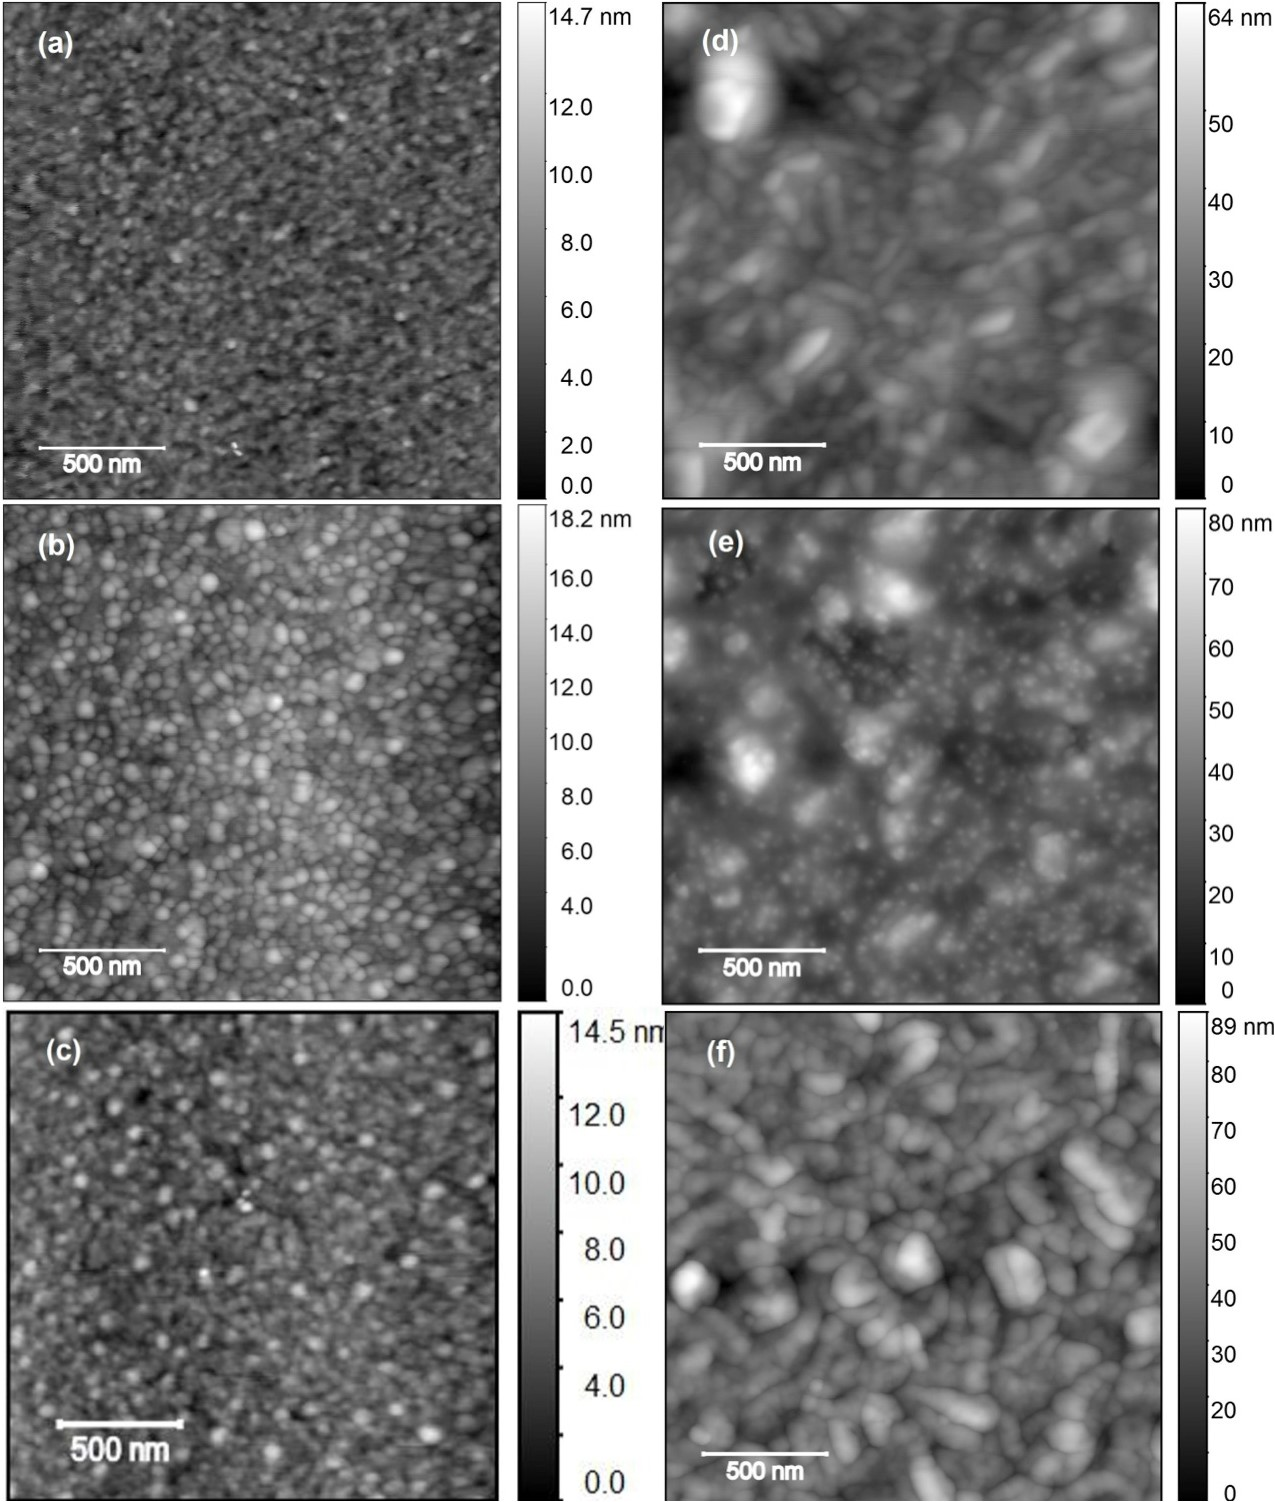
\includegraphics[width=1.0\textwidth]{Chapter-4/fig4_png}
	\caption{Representative AFM images of stainless steel 304 (left) and alumina (right) QCM electrodes after 1 h of oscillation in DI water (upper), −ND (middle) and +ND (lower) suspensions and then rinsing in DI water.}
	\label{fig4:AFM images}
\end{figure} 

Additional scanning electron microscopy (SEM) images (Figure 5) were recorded on the SS304 samples to further elucidate changes in the surface topology after exposure to NDs followed by rinsing in DI water. Alumina samples became rapidly charged upon an exposure to an electron beam (presumably due electrically isolating alumina layer still present on the electrode surface), preventing high quality SEM images from being recorded. Features associated with permanently adhering nanoparticles are present in the images for the samples exposed to ND. For the case of $−$ND exposure, the attached particles are clustered and the deposits are more uniformly distributed over the surface. The +ND exposure results in very sparse deposits, which form dendrite surface aggregates in regions where they are present.

\begin{figure}[hbtp]
	\centering
	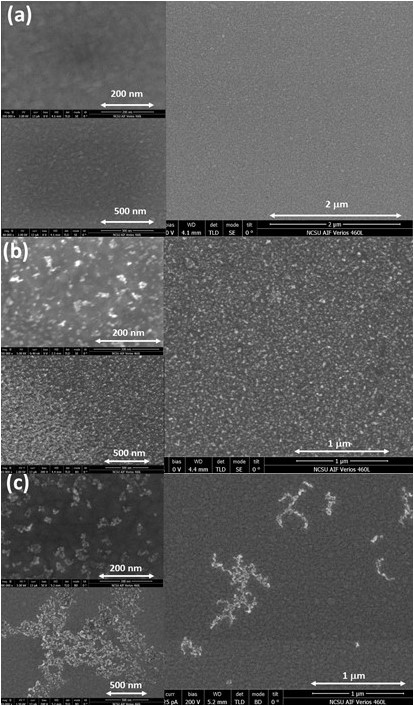
\includegraphics[width=0.8\textwidth]{Chapter-4/fig5_png}
	\caption{SEM images of SS304 QCM electrodes after oscillated in (a) water, (b) $−$ND, and (c) +ND suspensions for 1 h and then rinsed in DI water. See text for further details.}
	\label{fig5:AFM images}
\end{figure} 

The AFM and SEM data are consistent with the results from nanodiamond seeding literature [4.46], where it has been reported that the particle attachment density can, for example, vary from very low (108 cm−2) for hydrogen treated nanodiamonds (+ND) to very high (1011 cm−2) for oxidized nanodiamonds (−ND) on AlN substrates [4.47]. The data are also consistent with a report on a formation of ND clusters of ca. 23 nm in diameter on SiO\textsubscript{2} surfaces exposed to ND dispersions [4.48]. Clusters of this size are large enough to separate the surfaces employed for the Section ‘Macro-scale friction measurements’.

\begin{table}
	\caption{QCM frequency (+/$-$15 Hz) and resistance shifts (+/$−$1 Ω) in air before and after 60 min of oscillation in aqueous ND suspensions. The equivalent surface coverage of 25 nm clusters is also reported (+/−1 × 1010 clusters/cm2).}
	\label{table-one}
	\begin{center}
		\begin{tabular}{lcccccl}
			\toprule
			Sample & +ND immersion & & coverage & -ND immersion & & coverage\\
			
			\midrule
			& $\delta f (Hz)$ &  $\delta R (\Omega)$ & clusters/cm$^{2}$ & $\delta f (Hz)$ &  $\delta R (\Omega)$ & clusters/cm$^{2}$\\
			\midrule
			alumina & -8 & +15.5 & 0.7 $\times 10^{10}$ & -69 & -1.6 & 6.1 $\times 10^{10}$\\
			SS 304 	& -18 & -0.1 & 1.6 $\times 10^{10}$ & -25 & -0.1 & 2.2 $\times 10^{10}$\\
			
			\bottomrule
		\end{tabular}
	\end{center}
\end{table}

In order to characterize adhesion of NDs to surfaces quantitatively, the QCM frequencies and resistances were compared for crystals exposed to air before and after the exposure to the ND suspensions (followed by a rinse in pure water). The results, summarized in Table 1, exhibit a decrease in frequency after the exposure to the suspensions regardless of the ND surface charge sign. While some of the downward shifts in frequency may be attributable to a variation in the uptake of particulate and physisorbed species from air, the net mass increase is consistent with the addition of NDs in levels that exceed the mass of any material removed from the QCM electrode arising from the potentially erosive action of the ND. Consistent with the images, a definitive mass uptake is present for the alumina sample immersed in the −ND suspension. Resistance shifts were virtually zero for the stainless steel samples and consistent with the rigidly attached NDs. The increase in resistance for the alumina samples immersed in +ND is consistent with the presence of poorly attached layers that are slipping on the surface. This might be attributable to loosely attached NDs or physisorbed adsorbates, neither of which would be readily observed by AFM.

In order to convert the frequency shifts to particle density on the surface, we assume a cluster size of 25 nm and a packing fraction within the cluster of 0.7. The mass of each cluster would be [(25 nm/5 nm)3] × 0.7 (2.29 ×10−19 g/5 nm particle) = 2 × 10−17 g. A surface coverage of 1010 clusters per cm2 therefore has a mass per unit area of ρ2 = 2 × 10−7 g/cm2, which corresponds to a decrease in the resonant frequency of 11.3 Hz (cf.
Equation 3). For comparison, a monolayer of spherical 5 nm diamond nanoparticles packed in the closest hexagonal arrangement (assuming diamond bulk density of 3.5 g/cm3; mass per particle: 2.29 × 10−19 g) corresponds to 4.6 × 1012 ND/cm2, ρ2 = 1.058 × 10−6 g/cm2 and a decrease in the resonant frequency of 59.8 Hz.

Graphs of log(σ) vs log(scan size) obtained from the AFM images shown in Figure 4 are presented in Figure 6. Each data point represents an average of multiple locations on the surface. The slope of a linear fit in lower length scale gives the roughness exponent (H), and an exponential fit for the larger length scale gives the asymptotic value of σs, as described earlier.
All samples exhibited increases in σs after an oscillation in ND suspensions (Table 2). Alumina surfaces, however, exhibited greater increases in σs than SS304. Only the SS304 sample exposed to +ND exhibited a change in D, increasing from 2.2 to 2.3, which corresponds to a more jagged surface texture [4.30]. It is interesting to note that this is the only surface studied that exhibited a striking increase in friction upon an exposure to the NDs.


\begin{figure}[hbtp]
	\centering
	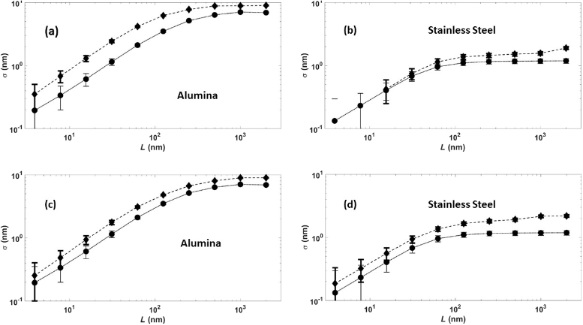
\includegraphics[width=0.8\textwidth]{Chapter-4/fig6_png}
	\caption{RMS roughness σ versus scan size L for QCM electrodes comprised of alumina (left) and stainless steel (right) after an oscillation for 1 h in DI water (solid lines) and after an oscillation for 1 h in suspensions of either positively (a),(b) or negatively (c),(d) (dashed lines) charged NDs. See text for details.}
	\label{fig6:AFM images}
\end{figure} 


All samples exhibited increases in σs after an oscillation in ND suspensions (Table 2). Alumina surfaces, however, exhibited greater increases in σs than SS304. Only the SS304 sample exposed to +ND exhibited a change in D, increasing from 2.2 to 2.3, which corresponds to a more jagged surface texture [4.30]. It is interesting to note that this is the only surface studied that exhibited a striking increase in friction upon an exposure to the NDs.

\begin{table}
	\caption{Saturated rms roughness σs (+/−0.1 nm) and fractal dimension D (+/−0.05) of QCM electrodes after 1 h of oscillation in DI water or ND suspensions.}
	\label{table-two}
	\begin{center}
		\begin{tabular}{lcccccl}
			\toprule
			Sample && Pure DI Water & & +ND suspension & & -ND immersion\\
			
			\midrule
			& $\sigma_{s} (nm)$ &$\mathit{D}$   &$\sigma_{s} (nm)$  & $\mathit{D}$   &  $\sigma_{s} (nm)$ &$\mathit{D}$ \\
			\midrule
			alumina &7.8 & 2.1 & 9.8 & 2.1 & 9.9 & 2.1\\
			SS 304 	&1.2 &2.2 & 1.6 & 2.3 & 2.4 & 2.2 \\
			
			\bottomrule
		\end{tabular}
	\end{center}
\end{table}


\section{QCM Measurements}

Frequency f and mechanical resistance R values of QCM relative to their initial values in air, \verb|f_air| and \verb|R_air|, are summarized in Figure 7. All QCM crystals were first exposed in DI water for 1 h followed by +ND or −ND dispersions for another 1 h and then returned to DI water for an additional 1 h. Fluid injections at 1 and 2 h in some cases caused temporary perturbations in f and R that serve as markers delineating the three regimes of exposure. All experiments were conducted at in at least triplicate using new QCM crystals, and only minor differences were observed between the individual runs.

\begin{figure}[hbtp]
	\centering
	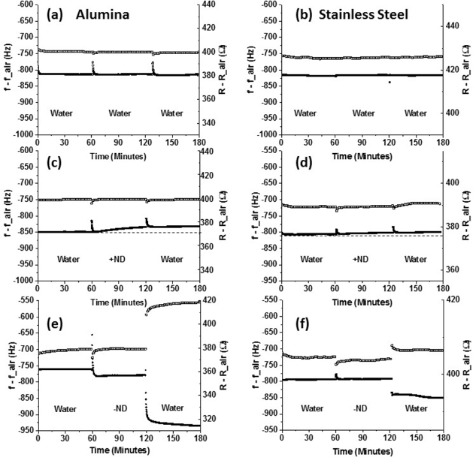
\includegraphics[width=0.8\textwidth]{Chapter-4/fig7_png}
	\caption{Time course of changes in mechanical resistance, R (top, open squares), and frequency f (bottom, filled squares), of QCM relative to air for SS304 (right) or alumna (left) electrode surfaces consequently exposed to DI water (a and b); +ND and water (c and d); −ND and water (e and f).}
	\label{fig7:AFM images}
\end{figure} 

Control runs in DI water (i.e., no ND exposure) are displayed in Figure 7a and 7b for the alumina and SS304 electrodes. Only minimal changes in f and R are observed in the control runs, apart from the momentary perturbations occurring at the time of pure water injections. Also, the drops in f and R relative to those recorded air are larger than the theoretical values for perfectly planar surfaces, −714 Hz and 300 Ω. These large experimental shifts are attributable to the surface roughness of the electrodes.

Changes in f and R for the samples exposed to ND suspensions were found to be dependent on the ND surface charge. Both the alumina and SS304 samples exhibit a slow, yet a small increase in f upon an exposure to +ND suspension (Figure 7c and 7d) that ceases upon re-entry of DI water. Given the AFM results indicating that both surfaces become slightly rougher upon an exposure to +ND, the upward trend does not appear to be attributable to the surface polishing but rather some modest erosive effects. Virtually no changes in the resistance to shear motion at the solid liquid interface were observed upon an introduction of the +ND. Such changes might result from loosely bound particles enabling some decoupling of the mass of the fluid surrounding the QCM with no significant reductions in the friction energy losses at the interface.

In contrast, significant changes in both f and R observed upon an exposure of both types of surfaces to −NDs and consequent rinsing in DI water (Figure 7e and 7f). Specifically, upon exposing the QCM to −ND suspension both f and R abruptly drop for the alumina sample while for the SS304 sample the frequency is essentially unchanged while R drops abruptly. Upon rinsing, an abrupt drop in f and a rise in R are observed for both surfaces. The QCM data provide a clear evidence of the −ND exposure permanently altering the both surfaces. These surface alterations appear to have a direct effect on the shear forces encountered at the solid–liquid interfaces. This global surface treatment may in fact provide a key piece of evidence to the fundamental mechanism underlying the friction reductions observed at the macroscale for the stainless steel and alumina surfaces immersed in −ND suspensions.

\section{Discussion}

The data reported here reveal key similarities and differences in both the macro- and nanotribological properties of stainless steel and alumina when exposed to ND aqueous dispersions. While Liu et al.’s suggestion that −ND dispersions are more likely to improve the tribological performance at the macroscale than the +ND dispersions [4.9] has been validated, the previous explanation of the underlying mechanism by strictly electrostatic appears to be somewhat simplistic within the context of simply comparing insulating alumina and conducting stainless steel surfaces.

For QCM electrodes coated with aluminum, the surface-exposed aluminum metal is readily oxidized to Al2O3 under ambient air. This surface layer of alumina is protecting the rest of metal from a further corrosion. In our experiments, the electrodes were additionally anodized for 3 min. This procedure is expected to yield approximately 50–100 nm thick Al2O3 layer. For Al2O3 is exposed to water one expect a formation of several aluminum hydroxide phases [4.49]. The presence of hydroxy (OH) groups on the alumina surface is affected by the oxide surface structure as well as other parameters with pH being the most important. Overall, the surface hydroxy groups determine electrostatic properties of the surface that, in turn, affect interactions of charged nanoparticles (NDs in this study) with the QCM alumina electrode.

In the past Cuddy et al. employed contact angle titration to determine Isoelectric points (IEPs) for five common (QCM) sensors [4.50]. Specifically, they reported a mildly basic IEP = 8.7 for Al2O3 sensors. Therefore, the QCM alumina surface is likely to be positively charged at the neutral pH of our experiments and this would explain a rapid uptake of negatively charged NDs on the electrode surface observed in our QCM experiments. Thus, this observation is in agreement with Liu’s electrostatic hypothesis [4.9]. We note that recently an electrostatic self-assembly seeding of monosized individual diamond nanoparticles (obtained by a detonation method) on silicon dioxide surfaces has been reported [4.51]. Although the latter study employed an aqueous dispersion of positively charged NDs, the silica surface is expected to be charged negatively at normal pH (IEP = 3.9, [4.50]) providing the same short-range electrostatic forces responsible for the ND surface self-assembly.

The EIP of SS304 surfaces, however, is somewhat acidic but could vary over a broader range from ca. 3.2 to 5.0 depending on the sample surface treatment according literature data summarized in [4.52]. Thus, at neutral pH or at a somewhat acidic pH of the DI water absorbing CO2 from air, the SS304 surface is expected to bare some negative change or no charge at all. Therefore, electrostatic interactions alone would not explain effects on −ND on tribological properties of SS304 surfaces.

One common feature observed in the data sets is that −ND dispersions produced through carboxylation consistently reduced the macroscopic friction coefficient relative to DI water by a factor of 2–5 for all stainless steel and alumina contacts studied and the value upon immersion consistently dropped into the range 0.05–0.1. QCM studies of stainless steel and alumina surfaces immersed in −ND dispersions meanwhile displayed behaviors consistent with a rapid uptake of −NDs, some slight but measurable increases in the surface roughness and distinct changes in the nature of the solid–liquid interfacial resistance to shear. These systems also exhibited an abrupt drop in f and an increase in R when re-exposed to pure DI water. The latter behavior is potentially explained by the suspended −ND nanoparticles acting as a lubricious slurry reducing resistance at the solid–liquid interface through potentially electrostatic repulsion with the rest of the −NDs in the surrounding suspension [4.20,43]. This suggestion, which is somewhat analogous to boundary lubrication and steric repulsion effects by mucinous glycoproteins boundary layers in aqueous biological settings [4.18], remains an intriguing possibility for the future investigations. The permanent changes observed in the surfaces morphology are likely associated with strong chemical attachment of −NDs in a manner distributed over the surface to form a more lubricous sliding interface than the bare surfaces alone.

It is notable that the literature on the contacts lubricated by aqueous ND suspensions for a range of materials reports the friction coefficients in the same range, 0.05–0.1, as observed here [4.2,7,8], while NDs similar to those employed here result in a markedly lower friction coefficients when treated with a dispersant so as to form colloids in oils [4.53]. This is consistent with a suggestion that the surface passivation treatments of NDs have great impact on the tribological properties. The notion is well known in the literature for diamond on diamond contacts in a variety of vacuum and humid environments [4.17,54-58]. The films of NDs strongly attached to surfaces are capable of providing both boundary lubrication and, potentially, a solid–liquid interface with a low resistance to shear. Therefore a custom design of nanolubrication systems by a proper chemical passivation of ND surfaces appears as a promising approach.

Hydroxylated NDs bearing a positive zeta potential in aquelus dispersion, produced no significant response in the frequency or resistance behavior of the QCM electrode covered with either alumina or SS304. While it is reasonable that the carboxylated −ND might exhibit more affinity to the alumina and stainless surfaces studied, one might conclude that the +ND suspensions would have little impact on the macroscale friction coefficients measured. But the friction increased significantly for the stainless steel materials. This may arise from corrosive and/or tribocorrosive effects at the macroscopic steel on steel interface being exacerbated by an abrasive action in the confined contact [4.59,60], a phenomena which was not probed by the AFM and QCM methods utilized here. It is notable that the changes in the QCM behavior upon immersion in +ND suspensions were very slow and gradual, in a stark contrast to the effects of the −ND suspensions. Detrimental wear at the macroscale might well out-pace any beneficial effects of ND for such liquid–solid interfaces.

We note that water was chosen as a liquid lubricant for this study so the results could be directly compared with preceding experiments of Liu et al. who employed QCM to investigate lubricating properties of aqueous suspensions of positively and negatively charged detonation nanodiamonds for gold electrode surfaces [4.9]. It is worthwhile to note that the methods described here are fully applicable to fluids other than water as long as the viscosity is sufficiently low for QCM to oscillate. Further studies will undoubtedly lead to a better understanding of third-body problems as well as improved design of the nanoparticle-based lubricants. Importantly, we have identified systems exhibiting beneficial, neutral, and detrimental tribology properties, facilitating additional experimental as well as theoretical studies from the first principles approach.

\section{Conclusion}

A comparative study of the nanoscale and macroscale tribological attributes of alumina and stainless steel surfaces immersed in positively (hydroxylated) or negatively (carboxylated) charged nanodiamond (ND) dispersion is reported here. The work has revealed key similarities and differences between the surfaces that are effectively or ineffectively lubricated by aqueous suspensions of ND. The principle observations and conclusions are as follows:

\begin{itemize}
	\item Immersion in −ND aqueous dispersion consistently resulted in a reduction in µk, for the stainless steel and alumina samples studied, falling by a factor of 2–5 to a steady state value in the range 0.05–0.1.
	
	\item Immersion in +ND aqueous dispersion consistently increased µk, for the stainless steel contacts and resulted in little to no increases for the alumina contacts.
	
	\item QCM and AFM measurements documented a rapid change in the surfaces of both alumina and stainless steel upon an exposure to −ND, consistent with a strong attachment of particles to the surfaces.
	
	\item The surfaces, upon uptake of ND, were characterized by a low resistance to shear at the interface between the solid and the aqueous −ND dispersion.
	
	\item Negligible polishing and/or abrasive effects were observed for QCM electrode surfaces after oscillating in either +ND or −ND dispersions for 1 h. The roughness of all the surfaces increased slightly upon an exposure to ND suspensions. This could be attributed to an attachment of NDs to the surface and/or some erosion effects.
	
	\item The +ND nanoparticles were not observed to rigidly adhere to the surfaces, for example, as a chemically bound adlayer, but some limited evidence was present for a loose attachment to alumina and very low coverages of dendritic aggregates on stainless steel.
	
	\item A suggested mechanism for the observations is that carboxylated −NDs in an aqueous dispersion form robust, lubricious film deposits on stainless steel and/or alumina surfaces that are both readily replenished by the surrounding suspensions and also glide through it with a relatively low resistance to shear, potentially because of the repulsive electrostatic forces between the individual particles.
	
\end{itemize} 

In summary, this study provides for atomic scale details associated with systems that exhibit radically different macro-scale tribological properties. It also reveals a broad class of materials that will be of great value in enabling theoretical efforts to predict and model complex lubricant interfaces.

\section{Acknowledgements}

This work was supported by NSF DMR1535082. SEM studies were performed at the Analytical Instrumentation Facility (AIF) at North Carolina State University, which is supported by the State of North Carolina and the NSF (Award Number ECCS-1542015). The AIF is a member of the North Carolina Research Triangle Nanotechnology Network (RTNN), a site in the National Nanotechnology Coordinated Infrastructure (NNCI). We are grateful to B. Acharya, D. Berman, D. Brenner, J. A. Harrison and K. J. Wahl for useful discussions. M. Chestnut and B. Vasconcelos de Farias are respectively thanked for assistance with recording of the electron micrographs and macroscale tribology measurements.


\addcontentsline{toc}{section}{{Chapter 5 References}}

\printbibliography[title=Chapter 5 References, keyword=five]
\chapter{AFM and QCM Study of the Nano-scale and Macro-scale Tribological Attributes of Polished and Unpolished, Rough Gold Surfaces Immersed in Functionalized Aqueous Nanodiamond Solutions}
\label{chap-six}










\addcontentsline{toc}{section}{{Chapter 6 References}}
\printbibliography[title=Chapter 6 References, keyword=six]
\chapter{Superparamagnetic Nanoparticle Mediated Dissipation in the Presence of External Magnetic Fields}
\label{chap-seven}

\section{Introduction}

for sure going to use Fe2O3

any other superparamagnetic particles worth acquiring



\subsection{Background Work}

Neel temperature

Curie Temperature

\subsection{Motivations}




\addcontentsline{toc}{section}{{Chapter 7 References}}
\printbibliography[title=Chapter 7 References, keyword=seven]
\chapter{Dissipation of Gaseous Species through Hydrogenated Graphene and Hydrogenated Graphene Oxide Layers atop Porous Media on QCM}
\label{chap-eight}





 \addcontentsline{toc}{section}{{Chapter 8 References}}
\printbibliography[title=Chapter 8 References, keyword=eight]
%\include{Chapter-9/Chapter-9}
%\printbibliography[title=Chapter 9 References, keyword=nine]
\chapter{Future Work}
\label{chap-ten}

\section{The State of the Art}

\section{Suggested Computational Studies}


\section{Suggested Experimental Work}




\addcontentsline{toc}{section}{{Chapter 10 References}}
\printbibliography[title=Chapter 10 References, keyword=ten]


%\restoregeometry

\begin{spacing}{1}
 \setlength\bibitemsep{11pt} %22pt = 2*11pt, where fontsize is 11pt

 \addcontentsline{toc}{chapter}{{\uppercase{\bibname}}} %\textorpdfstring and \uppercase needed due to hyperref package http://www.latex-community.org/forum/viewtopic.php?f=44&t=16601
% %\vspace{-0.5in}
\titleformat{\chapter}[display]{\bf\filcenter
}{\chaptertitlename\ \thechapter}{11pt}{\bf\filcenter}
\titlespacing*{\chapter}{0pt}{-0.5in-9pt}{22pt}

\printbibliography

\end{spacing}
%
%
%
\restoregeometry
%
\appendix
%
\newgeometry{margin=1in,lmargin=1.25in,footskip=\chapterfootskip, includehead, includefoot}


\chapter{ASAI - Adaptive Statistical Analysis for Images}
\label{Appendix A}


\section{Motivation for Development}

Surface roughness analysis, a staple technique in nano-tribology and the Krim nano-tribology group, though not particularly difficult for an individual image, quickly becomes time consuming and tedious as the number of images grows. Typically, using third-party software to assess the images, then using OriginPro (TM?) to plot and interpret those quantities, analysis of a single image would require a minimum of 10 minutes. Use of the ASAI package, written on the foundation of Krim Group roughness/fractal surface analysis principles, reduced the time cost for analysis of a single image to, on average, 10 seconds. In the event that there is a need to combine the roughness analysis output from multiple AFM images or to quickly change graph titles, time-savings are again added to the value of the ASAI system.

\section{Principles of Operation}


This code was developed around methods well-established in Dr. Krim's previous work including [refs for Krim surface roughness characterization]

Adaptive Analysis by Adj-R2 maximization

\section{Future Development Paths}

Generalizable to any matrix, square or otherwise....

\begin{figure}[hbtp]
	\centering
	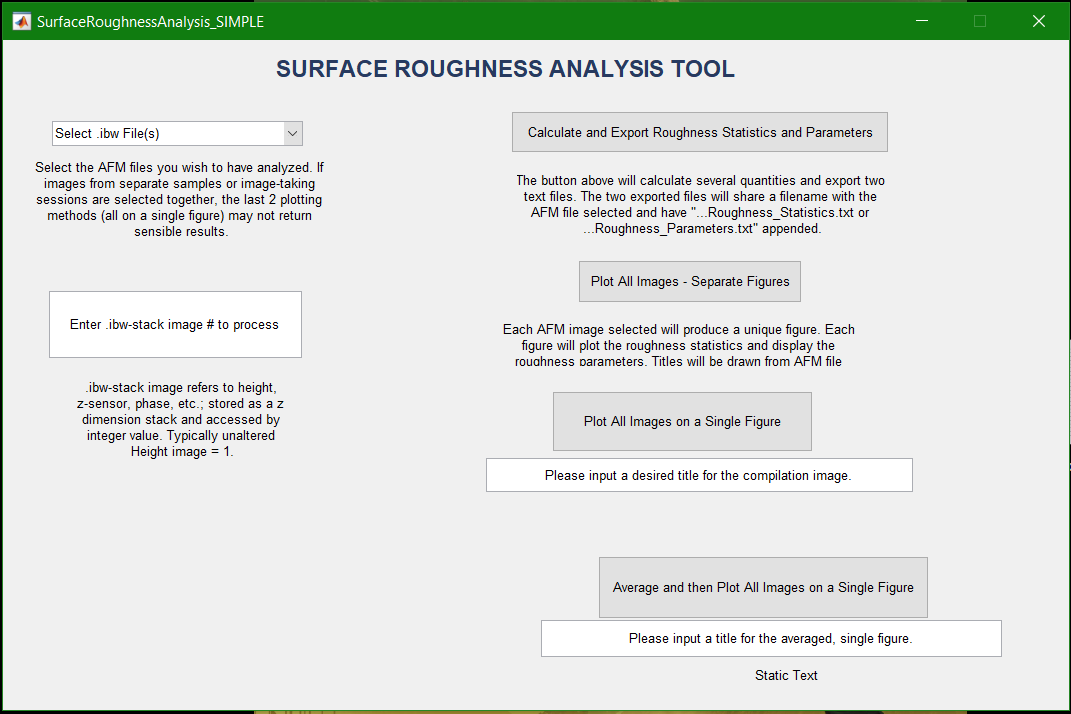
\includegraphics[width=1.0\textwidth]{Appendix-A/ASAI_GUI}
	\caption{ASAI, a MATLAB-based image analysis package, utilizes a simple graphical user interface (GUI) to provide a simple experience for users, regardless of programming skill.}
	\label{figA1: ASAI_GUI}
\end{figure} 


\section{ASAI Manual !!! Incomplete}

%%%%%%%%%%%%%%%%%%%%%%%%%%%%%%%%%%%%%%%%%%%%%%%%%%%%%%%%%
%%%%%%%%%%%%%%%%%%%%%%%%%%%%%%%%%%%%%%%%%%%%%%%%%%%%%%%%%

Adaptive Statistical Analysis for Images (ASAI) README

%%%%%%%%%%%%%%%%%%%%%%%%%%%%%%%%%%%%%%%%%%%%%%%%%%%%%%%%%
%%%%%%%%%%%%%%%%%%%%%%%%%%%%%%%%%%%%%%%%%%%%%%%%%%%%%%%%%

(c) 2017 North Carolina State University, Colin K Curtis, Jacqueline Krim

Author (code) =	Colin K Curtis
contact = 	colinkcurtis@gmail.com
github.com/colinkcurtis

Methods = Jacqueline Krim, citations: 
Panella, Krim. 1994.  "Adsorbate surface tension effects for isotherms
recorded on fractally rough surfaces"

Berman, Krim. 2012. "Impact of oxygen and argon plasma exposure on the
roughness of gold film surfaces"


%%%%%%%%%%%%%%%%%%%%%%%%%%%%%%%%%%%%%%%%%%%%%%%%%%%%%%%%%
%%%%%%%%%%%%%%%%%%%%%%%%%%%%%%%%%%%%%%%%%%%%%%%%%%%%%%%%%

Setup
%%%%%

There are several critical files which this package requires:

-SurfaceRoughnessAnalysis\_SIMPLE.fig  	(GUI component)
-SurfaceRoughnessAnalysis\_Simple.m    	(primary code)
-IBWread.m				(code for reading-in IBW files, a typical AFM output file type)				
-readIBWbinheader.m			(support code for IBWread.m)
-readIBWheaders.m			(support code for IBWread.m)

Ensure that all 5 objects, listed above, are placed into a single
directory. In the MATLAB IDE, 'Add' this directory/folder 'to the path'
so that MATLAB has all of the functional pieces within its scope.

If the IBW/image files which you wish to process are not located
in the directory along side the 5 aforementioned pieces of code,
"Add to path" the directory where your IBW/image files are stored.
If you do not add this directory to the MATLAB path, running the
program on a file outside the path will result in MATLAB errors.




%%%%%%%%%%%%%%%%%%%%%%%%%%%%%%%%%%%%%%%%%%%%%%%%%%%%%%%%%
%%%%%%%%%%%%%%%%%%%%%%%%%%%%%%%%%%%%%%%%%%%%%%%%%%%%%%%%%



%%%%%%%%%%%%%%%%%%%%%%%%%%%%%%%%%%%%%%%%%%%%%%%%%%%%%%%%%
%%%%%%%%%%%%%%%%%%%%%%%%%%%%%%%%%%%%%%%%%%%%%%%%%%%%%%%%%
%%%%%%%%%%%%%%%%%%%%%%%%%%%%%%%%%%%%%%%%%%%%%%%%%%%%%%%%%
%%%%%%%%%%%%%%%%%%%%%%%%%%%%%%%%%%%%%%%%%%%%%%%%%%%%%%%%%


\section{ASAI Code - Complete}

\begin{sloppypar}
\begin{lstlisting}

%
%%% --- GUI builder, from the MATLAB editor
%

function varargout = SurfaceRoughnessAnalysis_SIMPLE(varargin)
% SURFACEROUGHNESSANALYSIS_SIMPLE MATLAB code for
% SurfaceRoughnessAnalysis_SIMPLE.fig
%      SURFACEROUGHNESSANALYSIS_SIMPLE, by itself, creates a new
%      SURFACEROUGHNESSANALYSIS_SIMPLE or raises the existing singleton*.
%
%      H = SURFACEROUGHNESSANALYSIS_SIMPLE returns the handle to a new
%      SURFACEROUGHNESSANALYSIS_SIMPLE or the handle to the existing
%      singleton*.
%
%      SURFACEROUGHNESSANALYSIS_SIMPLE('CALLBACK',hObject,eventData,handles
%      calls the local function named CALLBACK in
%      SURFACEROUGHNESSANALYSIS_SIMPLE.M with the given input arguments.
%
%      SURFACEROUGHNESSANALYSIS_SIMPLE('Property','Value',...) creates a
%      new SURFACEROUGHNESSANALYSIS_SIMPLE or raises the existing
%      singleton*.  Starting from the left, property value pairs are
%      applied to the GUI before SurfaceRoughnessAnalysis_SIMPLE_OpeningFcn
%      gets called.  An unrecognized property name or invalid value makes
%      property application stop.  All inputs are passed to
%      SurfaceRoughnessAnalysis_SIMPLE_OpeningFcn via varargin.
%
%      *See GUI Options on GUIDE's Tools menu.  Choose "GUI allows only one
%      instance to run (singleton)".
%
% See also: GUIDE, GUIDATA, GUIHANDLES

% Edit the above text to modify the response to help
% SurfaceRoughnessAnalysis_SIMPLE

% Last Modified by GUIDE v2.5 28-Nov-2016 16:13:05

% Begin initialization code - DO NOT EDIT
gui_Singleton = 1;
gui_State = struct(		'gui_Name',       mfilename, ...
'gui_Singleton',  gui_Singleton, ...
'gui_OpeningFcn', @SurfaceRoughnessAnalysis_SIMPLE_OpeningFcn, ...
'gui_OutputFcn',  @SurfaceRoughnessAnalysis_SIMPLE_OutputFcn, ...
'gui_LayoutFcn',  [] , ...
'gui_Callback',   []);
if nargin && ischar(varargin{1})
gui_State.gui_Callback = str2func(varargin{1});
end

if nargout
[varargout{1:nargout}] = gui_mainfcn(gui_State, varargin{:});
else
gui_mainfcn(gui_State, varargin{:});
end
% End initialization code - DO NOT EDIT

% --- Executes just before SurfaceRoughnessAnalysis_SIMPLE is made visible.
function SurfaceRoughnessAnalysis_SIMPLE_OpeningFcn(hObject, eventdata,...
handles, varargin)
% This function has no output args, see OutputFcn. hObject    handle to
% figure eventdata  reserved - to be defined in a future version of MATLAB
% handles    structure with handles and user data (see GUIDATA) varargin
% command line arguments to SurfaceRoughnessAnalysis_SIMPLE (see VARARGIN)

% Choose default command line output for SurfaceRoughnessAnalysis_SIMPLE
handles.output = hObject;

% Update handles structure
guidata(hObject, handles);

% UIWAIT makes SurfaceRoughnessAnalysis_SIMPLE wait for user response (see
% UIRESUME) uiwait(handles.figure1);

% --- Outputs from this function are returned to the command line.
function varargout = SurfaceRoughnessAnalysis_SIMPLE_OutputFcn(hObject, ...
eventdata, handles) 
% varargout  cell array for returning output args (see VARARGOUT); hObject
% handle to figure eventdata  reserved - to be defined in a future version
% of MATLAB handles    structure with handles and user data (see GUIDATA)

% Get default command line output from handles structure
varargout{1} = handles.output;

% --- Executes on selection change in popupmenu1.
function popupmenu1_Callback(hObject, eventdata, handles)

global A
global AFMMetaData
global FileName
global IBWFiles
global Space

Space = ' '; %Just a space used in glueing together strings throughout 
...the program!

% The lines below take important information from the AFM file, such as
% file name, Scan Size (physical and # pixels), and Imaging mode, and save
% them for calculation or later use on the graphs to be plotted
[FileName, PathName, filterindex] = uigetfile('*.ibw',... 
'Select the ibw file', 'MultiSelect','on');
if ischar( FileName ), FileName = { FileName };  % for uigetfile,
end										% single file read-in is trouble

A = length(FileName);        % A variable we use in for loops to follow
IBWFiles = cell(1,A);       % This will hold the image data itself!!!

for i= 1:A                % Look through all of the files selected above

Q = FileName{i};        % Assign the filename to variable Q  
P = IBWread(Q);         % This fcn reads in and assigns ibw files to P
IBWFiles{i} = P;        % Creates a cell array of all the read-in files
tempWaveNotes = P.WaveNotes;  % this

AFMMetaData{i} = textscan(tempWaveNotes, '%s','delimiter', '\n');

%     assignin('base','IBWFiles',IBWFiles);       % Adds the cell array
%     just created to the workspace assignin('base','FileName',FileName);
end

%    assignin('base','AFMMetaData',AFMMetaData);

if isequal(FileName,0) % in case no file is selected, a msg is displayed
disp('User did not select files')

else                    % the filenames of the files read in are displayed
disp(['user selected the .ibw file(s):', fullfile(PathName, FileName)])
end


% --- Executes during object creation, after setting all properties.
function popupmenu1_CreateFcn(hObject, eventdata, handles)

if ispc && isequal(get(hObject,'BackgroundColor'), ... 
get(0,'defaultUicontrolBackgroundColor'))
set(hObject,'BackgroundColor','white');
end


function edit2_Callback(hObject, eventdata, handles)

get(hObject,'String');


% --- Executes during object creation, after setting all properties.
function edit2_CreateFcn(hObject, eventdata, handles)

if ispc && isequal(get(hObject,'BackgroundColor'), ... 
get(0,'defaultUicontrolBackgroundColor'))
set(hObject,'BackgroundColor','white');
end


function edit3_Callback(hObject, eventdata, handles)

get(hObject,'String');


% --- Executes during object creation, after setting all properties.
function edit3_CreateFcn(hObject, eventdata, handles)

if ispc && isequal(get(hObject,'BackgroundColor'), ...
get(0,'defaultUicontrolBackgroundColor'))
set(hObject,'BackgroundColor','white');
end



function edit5_Callback(hObject, eventdata, handles)

get(hObject,'String');

% --- Executes during object creation, after setting all properties.
function edit5_CreateFcn(hObject, eventdata, handles)

if ispc && isequal(get(hObject,'BackgroundColor'), ...
get(0,'defaultUicontrolBackgroundColor'))
set(hObject,'BackgroundColor','white');
end

%
%%% ROUGHNESS STATISTICS AND ROUGHNESS PARAMETER CALCULATION AND FILE
%%% EXPORT
%
function pushbutton1_Callback(hObject, eventdata, handles)

format longeng    % makes it so we can see numbers which are different ...
% by orders of magnitude

global A
global AllImageStats
global AFMMetaData
global AllExpFitCoefficients
global AllLinFitCoefficients
global AllRoughnessParameters
global DataForFitting
global FileName
global FirstExpFit
global FirstExpFitOptions
global IBWFiles
global LastLinearPoint
global LinFit
global PhysicalScanSize
global Pixels
global SquareRootofLastWeight
global y0Start

AllImageStats = cell(1,A);     % pre-allocates a cell array which will 
% store the calculated length/RMS matrices
DataFileHeader = cell(1,3); %This will be the header for the 
%"____statistics.txt" export text file
DataFileHeader = {'Length(A)','RMS Roughness(A)','STD of Roughness(A)'};
ImageSelect = get(handles.edit2, 'string');
ImageSelect = str2double(ImageSelect);
Pixels = zeros(1,A);
VarianceOfLogRMSValues = 1;

disp '***Roughness Analysis Has Begun***'

for i = [1:A]                       
tempCELL = IBWFiles{i};       % picks out a single image file-set 
% from the cell array

PickHeight = tempCELL.y; % picks out all of the height data 
% (for all of the available types, 
%phase, amplitude, height, etc) from the file

PickImage = PickHeight(:,:,ImageSelect);  % selects the 6th image, 
%in my case the modified height, THIS NEEDS TO BE USER-INPUT

Pixels(1,i) = length(PickImage);     % # of pixels for a square image 
% in EACH DIMENSION

N = log(Pixels(1,i))/log(2);         % This will control the outer-most
% for loop for each image, below

tempStringforPhysicalScanSize= AFMMetaData{i}{1}{1};  
% This will go into the AFM-file meta-data to find physical image size

clippedString = strrep(tempStringforPhysicalScanSize,'ScanSize: ','');

PhysicalScanSize = 10e9*str2double(clippedString); 
% Gives the square-dimension of the image in Angstroms

AngstromLength = zeros(N,1);    
% pre-allocate a matrix to hold length values in Angstroms

RMSValues = zeros(N,1);         
% pre-allocate a matrix to hold RMS Roughness values for each length-scale

LogAngstromLength = zeros(N,1);

LogRMSValues = zeros(N,1);

LogRMSWeights = zeros(N,1);

LogSTD = zeros(N,1);

STD = zeros(N,1);               
% pre-allocate a matrix to hold the uncertainty for each RMS Roughness value

for j = [1:N]                 
% this outer loop will reset for each image selected

PixelsPerSquare = 2^j;      
% determines the number of pixels (for each dimension) to examine

NumberOfValuesToAVG = (Pixels(1,i)/PixelsPerSquare)^2;    
% With each new length scale, the number of values changes as x^2

RMSHolder = zeros(NumberOfValuesToAVG,1);       
% pre-allocates a matrix in which the STD from each small square

m = 1; % is saved until they can be averaged and STD calculated                                                 

ADD = 2^j-1;        
% ADD is an incrementer which adjusts to the size of the box being
%  used for STD calculations, below

for k = [1:PixelsPerSquare:(Pixels(1,i)-PixelsPerSquare+1)]          
%in the x-direction, this loop takes us across the pixels
%by bits = to the square size defined prev as "pixel per square"
incrementk = k + ADD;                                                     

for l = [1:PixelsPerSquare:(Pixels(1,i)-PixelsPerSquare+1)]          
% runs through the y values    
incrementl = l + ADD;                
RMSHolder(m) = std2(PickImage(k:incrementk,l:incrementl));    
% The heart of things: finds the std for each small square
m = m + 1;
%increments the list of STDs forward to save the next value
end
end

StdOfRMS = std(RMSHolder)*1e10;         
% Finds the STD/uncertainty for all the little-square calculations
RMSMean = mean(RMSHolder)*1e10;         
% averages the measurements from each small square
STD(j) = StdOfRMS;                      
% Stores the avg STD value in a vector for calculation of LogSTD 
% in the next line
LogSTD(j) = STD(j)/(RMSMean*log(10));   
% This is the fractional uncertainty of LogRMSValues, below   
RMSValues(j) = RMSMean;                 
%Adds to the average from above to a list which saves 
% the values across length scales, for each image
LogRMSValues(j) = log10(RMSMean);       
% this will be the y-value we use for "roughness statistics" and 
%calculating roughness parameters

tempAngstromLength =PhysicalScanSize*(PixelsPerSquare/Pixels(1,i));  
% need to turn pixel values into real length values!
AngstromLength(j) = tempAngstromLength;                               
% creates a list of the real lengths we have just calculated
LogAngstromLength(j) = log10(tempAngstromLength);                     
% we want log-log for roughness parameter calculations, 
% this is the x-values vector

if j ~= N
VarianceOfLogRMSValues = LogSTD(j)*LogSTD(j);  
% We calculate the weights for each point for the final fit
LogRMSWeights(j) = 1 / VarianceOfLogRMSValues; 
% The weight, for each data point, is  1 / variance
else
tempFit = fitlm(LogAngstromLength,LogSTD);   
% so... above we could find the weights for fitting quite easily

tempSlope = tempFit.Coefficients{2,1};       
% but the last RMS roughness measurement, of the ENTIRE AFM image

tempy0 = tempFit.Coefficients{1,1};          
% produces only ONE value. Thus, there is no obvious 
% STD/uncertainty to use!

SquareRootofLastWeight = tempSlope(1,1)*LogAngstromLength(j)+tempy0(1,1); 

LogSTD(j) = SquareRootofLastWeight;          
% So, here we fit the uncertainties of all of the 
% smaller RMS roughness values

LastWeight = SquareRootofLastWeight^2;       
% which were calculated, used to extrapolate what might expect

LogRMSWeights(j) = 1 / LastWeight;           
% The uncertainty of the last single RMS roughness measurements
% to be
end

XandYandZ = [AngstromLength RMSValues STD LogAngstromLength ...
LogRMSValues LogSTD LogRMSWeights]; 
% creates a 6-column matrix with important values
y0Start = LogRMSValues(end);         
% this is  used to give the exponential fit a place to begin 
% its search for a y-intercept

end

OutputTemp1 = FileName{i};
OutputTemp1 = OutputTemp1(1:end-4);
NameForTextFile = sprintf('%s_Roughness_Statistics.txt',OutputTemp1);
AllImageStats{1,i} = {NameForTextFile; DataFileHeader; XandYandZ};              
% Adds the 3-column list to a cell array to store for all selected
% images

%assignin('base','AllImageStats',AllImageStats); % DIAGNOSTIC: Saves
%the above stat lists for all of the images to the workspace
% useful as a diagnostic tool
end

LS = 'Length Scale [Angstroms]', RR = 'RMS Roughness [Angstroms]', ...
STDRR = 'STD of RMS Roughness [Angstroms]';
LOGLS = 'log(Length Scale)', LOGRR = 'log(RMS Roughness)', ...
STDLOGRR = 'STD of log(RMS Roughness)';

for i = [1:A]
tempName = AllImageStats{i}{1};
tempData = AllImageStats{i}{3};

tempRoughnessStatisticsExportFile = fopen(tempName,'w');
fprintf(tempRoughnessStatisticsExportFile, '%s\n', tempName);  
fprintf(tempRoughnessStatisticsExportFile, ...
'%s %4s %4s %4s %4s %4s\n',LS,RR,STDRR,LOGLS,LOGRR,STDLOGRR);
fprintf(tempRoughnessStatisticsExportFile, ...
'%2.1f %20.1f %30.1f %10.1f %10.1f %10.1f\n',tempData');
fclose(tempRoughnessStatisticsExportFile);
end

disp '**Done Computing Roughness Statistics**'

AllExpFitCoefficients = cell(2,A);  
% We will need to store and re-use the fitting parameters
AllLinFitCoefficients = cell(1,A);  
% for calculations of Roughness Parameters as well as 
AllRoughnessParameters = cell(1,A); 
% plotting figures in functions to follow

FirstExpFit = fittype('y0+a*exp(b*x)','independent','x','dependent','y','coefficients',{'y0','a','b'});

FirstExpFitOptions = fitoptions(FirstExpFit);
%FirstExpFitOptions.Algorithm = 'Levenberg-Marquardt';
%FirstExpFitOptions.Robust = 'LAR';
FirstExpFitOptions.StartPoint = [y0Start -150 0.1];   
% the start point, and lower upper bounds for fitting

FirstExpFitOptions.Lower = [0 -300 -5];               
% were determined by using OriginPro to fit several plots of the Roughness Statistics data                                                    

FirstExpFitOptions.Upper = [5  0 0];
FirstExpFitOptions.MaxFunEvals = 50000;
FirstExpFitOptions.MaxIter = 50000;

LastLinearPoint = zeros(A,1);  
% pre-allocates a vector to hold the points where the fit should 
% switch over from linear to exponential, for different AFM images

for i = [1:A]

BREAK = 0;
N = AllImageStats{i}{3};    
% this is for convenience so the global variable 
% does not keep getting called
tempLength = length(N(:,1));  
% we previously calculated the roughness 
% statistics with # rows = tempLength
testOnesVector = ones(tempLength,1); 
%diagnostic vector for tinkering with weights 4 the fitting procedures

DataForFitting = zeros(tempLength,2); 
% pre-allocate a matrix of width 3 and length tempLength 

DataForFitting(:,1) = N(:,4);  
% this column = Log (Length Scale [A])

DataForFitting(:,2) = N(:,5); 
% this column = Log (RMS Roughness [A])

ExpFitAdjRHolder = zeros(tempLength,1);

for k = [2:tempLength-2] 

%FirstExpFitOptions.Weights = testOnesVector(end-k-1:end,1);
FirstExpFitOptions.Weights = AllImageStats{1,i}{3}(end-k:end,7);
[ExpFit, GoF] = fit(DataForFitting(end-k:end,1), ...
DataForFitting(end-k:end,2), FirstExpFit, FirstExpFitOptions);
AdjR2 = GoF.adjrsquare;
ExpFitAdjRHolder(k) = AdjR2;

if ExpFitAdjRHolder(k) < ExpFitAdjRHolder(k-1)

FirstExpFitOptions.Weights = AllImageStats{1,i}{3}(end-k-1:end,7);       
[ExpFit, GoF2] = fit(DataForFitting(end-k-1:end,1), ...
DataForFitting(end-k-1:end,2), FirstExpFit, FirstExpFitOptions);
AdjR2_2 = GoF2.adjrsquare;
ExpFitAdjRHolder(k+1) = AdjR2_2;

if AdjR2_2 < ExpFitAdjRHolder(k-1)

FirstExpFitOptions.Weights = ...
AllImageStats{1,i}{3}(end-k:end,7);
[ExpFit, GoF] = fit(DataForFitting(end-k:end,1), ...
DataForFitting(end-k:end,2), FirstExpFit, ...
FirstExpFitOptions);
BREAK = 1;          
end
end

if BREAK == 1
break
end

FirstExpPoint = tempLength - k + 1;
LastLinearPoint(i,1) = FirstExpPoint;
temp4 = tempLength - FirstExpPoint + 1;
end

ExpFitCoefficients = coeffvalues(ExpFit); 
% Here we pull out the coeffcients from the exponential fit, above
y0 = ExpFitCoefficients(1);
a = ExpFitCoefficients(2);
b = ExpFitCoefficients(3);
ExpFitError = GoF.sse;

ExpRange = temp4;
ExpFitConfidenceInterval = confint(ExpFit);
BOTTOM = ExpFitConfidenceInterval(1,1);
TOP = ExpFitConfidenceInterval(2,1);
ConfidenceIntervalRange = TOP - BOTTOM;
tvalue = tinv(0.95,ExpRange);

ExpFitYIntercept = ExpFitCoefficients(1);    
ExpFitYInterceptError = sqrt(ExpRange)*ConfidenceIntervalRange/tvalue;
y0error = ExpFitYInterceptError;    
ExpFitYInterceptPartialError=(ExpFitYInterceptError/ExpFitYIntercept)^2;

AllExpFitCoefficients {1,i} = {y0;a;b}; 
% We now store the coefficients from the exponential 
% fit for later calculation and plotting

AllExpFitCoefficients {2,i} = {y0error;ExpFitError};

assignin('base','AllExpFitCoefficients',AllExpFitCoefficients); 
% DIAGNOSTIC

LinFit = fitlm(DataForFitting(1:LastLinearPoint(i,1),1),...
DataForFitting(1:LastLinearPoint(i,1),2),'Weight', ... 
AllImageStats{1,i}{3}(1:LastLinearPoint(i,1),7));

LinearYIntercept = LinFit.Coefficients{1,1};
LinearYInterceptError = LinFit.Coefficients{1,2};
LinearYInterceptPartialError = ...
(LinearYInterceptError/LinearYIntercept)^2;

LinearSlope = LinFit.Coefficients{2,1};
LinearSlopeError = LinFit.Coefficients{2,2};
LinearSlopePartialError = (LinearSlopeError/LinearSlope)^2;
AllLinFitCoefficients{1,i} = {LinearSlope; LinearSlopeError ; ...
LinearYIntercept ; LinearYInterceptError};
% assignin('base','AllLinFitCoefficients', AllLinFitCoefficients);

XIntercept = ((y0)-LinearYIntercept)/LinearSlope;
XInterceptError = XIntercept*sqrt(LinearSlopePartialError + ...
LinearYInterceptPartialError + ExpFitYInterceptPartialError);

%BELOW WE CALCULATE THE THREE ROUGHNESS PARAMETERS

FractalDimension = 3 - LinearSlope;
FractalDimensionError = FractalDimension*(LinearSlopeError/LinearSlope);

SaturationRoughness = 10^(y0);
SaturationRoughnessError = SaturationRoughness * ...
(ExpFitYInterceptError / ExpFitYIntercept);

CorrelationLength = 10^XIntercept;
CorrelationLengthError = CorrelationLength * ...
(XInterceptError / XIntercept);

ThreeParameters = [FractalDimension SaturationRoughness ...
CorrelationLength];
ThreeParametersError = [FractalDimensionError SaturationRoughnessError ...
CorrelationLengthError];
%assignin('base','ThreeRoughnessParameters',ThreeParameters);

OutputTemp2 = FileName{i};
OutputTemp2 = OutputTemp2(1:end-4);
RoughnessParameterFileName = sprintf('%s_Roughness_Parameters.txt',...
OutputTemp2);
AllRoughnessParameters{1,i} = {RoughnessParameterFileName; ...
ThreeParameters; ThreeParametersError};

%assignin('base','DataForFitting',DataForFitting) % DIAGNOSTICS
%assignin('base','LinFit',LinFit) assignin('base','ExpFit',ExpFit)
end  

FD = 'Fractal Dimension', SR = 'Saturation Roughness [Angstroms]', ...
CL = 'Correlation Length [Angstroms]';

for i = [1:A]

tempName2 = AllRoughnessParameters{i}{1};
tempData2 = AllRoughnessParameters{i}{2};

tempRoughnessParameterExportFile = fopen(tempName2,'w'); 
fprintf(tempRoughnessParameterExportFile, '%s\n', tempName2);  
fprintf(tempRoughnessParameterExportFile, '%s %2s %2s\n',FD,SR,CL); 
fprintf(tempRoughnessParameterExportFile, '%.1f %20.1f %30.1f',...
tempData2);
fclose(tempRoughnessParameterExportFile);
end
disp '***Done Computing Roughness Parameters***'

%
%%% --- Display each AFM image's Roughness Report in an individual figure
%

function pushbutton3_Callback(hObject, eventdata, handles)

global A
global AFMMetaData
global AllExpFitCoefficients
global AllImageStats
global AllLinFitCoefficients
global AllRoughnessParameters
global FileName
global LastLinearPoint
global Pixels
global Space
global y0

clippedString = '';

for i = [1:A]

N = AllImageStats{i}{3}; 
tempLength = length(N(:,1));

DataForFitting2 = zeros(tempLength,3);
DataForFitting2(:,1) = N(:,4);
DataForFitting2(:,2) = N(:,5);
DataForFitting2(:,3) = N(:,6);    

LinSlope = AllLinFitCoefficients{1,i}{1};
LinYIntercept = AllLinFitCoefficients{1,i}{3};

y0 = AllExpFitCoefficients{1,i}{1,1}; a = ...
AllExpFitCoefficients{1,i}{2,1}; b = AllExpFitCoefficients{1,i}{3,1};

XforLinear = DataForFitting2(1:LastLinearPoint(i,1),1);
YforLinear = LinYIntercept + LinSlope*XforLinear;

XforExp = DataForFitting2(LastLinearPoint(i,1):end,1);
YforExp = y0 + a*exp(b*XforExp);

%%%Now we plot our data!

figure();
tempName2 = FileName{i};
tempName2 = tempName2(1:end-4); 

% Below is a text box which will display the title of the sample/image
GraphTitle = cat(2,'Roughness Analysis for: ',tempName2,'');
TitleNotes = annotation('textbox',...
[0.195 0.84 0.64 0.075],...
'String',{GraphTitle},...
'FontSize',14,...
'FontName','Constantina',...
'LineStyle','-',...
'EdgeColor',[0 0 0],...
'LineWidth',0.01,...
'BackgroundColor',[1 1 1],...
'Color',[0.1 0.1 0.1],...
'Interpreter', 'none',...
'FontWeight', 'bold',...
'HorizontalAlignment','center',...
'FitBoxToText','on');

FractalDimension = AllRoughnessParameters{1,i}{2,1}(1,1);
FractalDimension = num2str(FractalDimension);
FractalDimension = FractalDimension(1:end-2);

FractalDimensionError = AllRoughnessParameters{1,i}{3,1}(1,1);
FractalDimensionError = ceil(FractalDimensionError/10^floor...
(log10(FractalDimensionError)))...
*10^floor(log10(FractalDimensionError)); % salt to suit...

FractalErrorInfo = num2str(FractalDimensionError);
FractalErrorInfo = cat(2,'(',FractalErrorInfo,')');
FractalInfo = 'Fractal Dimension: ';
FractalInfo = ...
cat(2,FractalInfo, FractalDimension,Space,FractalErrorInfo);

SatRuffError = AllRoughnessParameters{1,i}{3,1}(1,2);
SatRuffError = ceil(SatRuffError/10^floor(log10(SatRuffError)))...
*10^floor(log10(SatRuffError)); % salt to suit...

SatRuffErrorInfo = num2str(SatRuffError);
SatRuffErrorInfo = cat(2,'(',SatRuffErrorInfo,')');
SatRuff = AllRoughnessParameters{1,i}{2,1}(1,2);
SatRuff = num2str(SatRuff);
SatRuff = SatRuff(1:end-3);
SatRuffInfo = 'Saturation Roughness: ';
SatRuffInfo = ...
cat(2,SatRuffInfo, SatRuff,Space,SatRuffErrorInfo,' [A]');

CorrLengthError = AllRoughnessParameters{1,i}{3,1}(1,3);
CorrLengthError = ceil(CorrLengthError/10^floor...
(log10(CorrLengthError)))*10^floor(log10(CorrLengthError)); 
CorrLengthErrorInfo = num2str(CorrLengthError);
CorrLengthErrorInfo = cat(2,'(',CorrLengthErrorInfo,')');
CorrLength = AllRoughnessParameters{1,i}{2,1}(1,3);
CorrLength = num2str(CorrLength);
CorrLength = CorrLength(1:end-4);
CorrLengthInfo = 'Correlation Length: ';
CorrLengthInfo = cat(2, CorrLengthInfo, CorrLength, ...
Space, CorrLengthErrorInfo,' [A]'); 

[PhysicalImageSize,ImageResolution] = ImageSizeProperties(Pixels,...
AFMMetaData);

%%%
ImageNotes = annotation('textbox',...
[0.62 0.08 0.1 0.3],...
'String',{PhysicalImageSize ImageResolution Space ...
FractalInfo SatRuffInfo CorrLengthInfo },...
'FontSize',14,...
'FontName','Constantina',...
'LineStyle','-',...
'EdgeColor',[0 0 0],...
'LineWidth',0.1,...
'BackgroundColor',[1 1 1],...
'Color',[0.1 0.1 0.1],...
'FitBoxToText','on');

plot(XforLinear, DataForFitting2(1:LastLinearPoint(i,1),2),'o'); ...
hold on;
plot(XforLinear,YforLinear,'b'), hold on;  
plot(XforExp, YforExp,'g'), hold on;
plot(XforExp, DataForFitting2(LastLinearPoint(i,1):end,2),'x');

errorbar(DataForFitting2(:,1),DataForFitting2(:,2), ...
DataForFitting2(:,3),'r.');

grid on;
axis([1.5 ceil(DataForFitting2(end,1)*10)/10 0 ...
DataForFitting2(end,2)+DataForFitting2(end,2)/4]);
xlabel('Log( LengthScale [A] )','FontWeight','bold','FontName',...
'Constantina','FontSize',16); 
ylabel('Log( RMS Roughness [A] )','FontWeight','bold','FontName',...
'Constantina','FontSize',16);
end

% --- Plot Data from ALL AFM IMAGES SELECTED on a Single Figure
%
function pushbutton4_Callback(hObject, eventdata, handles)
% hObject    handle to pushbutton4 (see GCBO) eventdata  reserved - to be
% defined in a future version of MATLAB handles    structure with handles
% and user data (see GUIDATA)

global A
global AFMMetaData
global AllLinFitCoefficients
global AllExpFitCoefficients
global AllImageStats
global AllRoughnessParameters
global LastLinearPoint
global Pixels
global Space
global y0


SumOfWeightedSatRuffs = 0;
SumOfSatRuffWeights = 0;

SumOfWeightedCorrLengths = 0;
SumOfCorrLengthWeights = 0;

SumOfWeighteds = 0;
SumOfFractalDimensionWeights = 0;


clippedString = '';
CorrLengthError = 0;
CurrentCorrLength = 0;
CurrentCorrLengthError = 0;
CurrentCorrLengthWeight = 0;
CurrentDf = 0;
CurrentDfError = 0;
CurrentDfWeight = 0;
CurrentSatRuff = 0;
CurrentSatRuffError = 0;
CurrentSatRuffWeight = 0;
DfError = 0;
FractalDimensionWeightedAVGError = 0;
SatRuff = 0;
SatRuffError = 0;
sqrtA = sqrt(A);
HolderForSumOfCorrLengthWeights = 0;
SumOfDfWeights = 0;
SumOfSatRuffWeights = 0;
SumOfFractalDimensions = 0;
SumOfCorrLengths = 0;
SumOfCorrLengthsError = 0;
TotalLinSlope = 0;
TotalLinSlopeError = 0;
TotalLinYIntercept = 0;
TotalLinYInterceptError = 0;
SumOfSatRuffs = 0;
SumOfSatRuffsError = 0;
TotalYDataForFitting = zeros(length(AllImageStats{1}{3}),1);
TotalYErrorDataForFitting = zeros(length(AllImageStats{1}{3}),1);
SumOfCorrLengthWeights = 0;
HolderForSumOfCorrLengths = 0;
CL = 0;
CLW = 0;

for i = [1:A]

N = AllImageStats{i}{3}; 
tempLength = length(N(:,1));

DataForFitting2 = zeros(tempLength,3);
DataForFitting2(:,1) = N(:,4);
DataForFitting2(:,2) = N(:,5);
DataForFitting2(:,3) = N(:,6);    

LinSlope = AllLinFitCoefficients{1,i}{1};
TotalLinSlope = TotalLinSlope + LinSlope;
LinSlopeError = AllLinFitCoefficients{1,i}{2};
TotalLinSlopeError = TotalLinSlopeError + LinSlopeError;

LinYIntercept = AllLinFitCoefficients{1,i}{3};
TotalLinYIntercept = TotalLinYIntercept + LinYIntercept;
LinYInterceptError = AllLinFitCoefficients{1,i}{4};
TotalLinYInterceptError = TotalLinYInterceptError + LinYInterceptError;

y0 = AllExpFitCoefficients{1,i}{1,1}, ...
a = AllExpFitCoefficients{1,i}{2,1}, ...
b = AllExpFitCoefficients{1,i}{3,1};

XforLinear = DataForFitting2(1:LastLinearPoint(i,1),1);
YforLinear = LinYIntercept + LinSlope*XforLinear;

XforExp = DataForFitting2(LastLinearPoint(i,1):end,1);
YforExp = y0 + a*exp(b*XforExp);

[CL,CLW] = SumOfWeightedCorrelationLengthsAndWeights ...
(i, AllRoughnessParameters)
SumOfWeightedCorrLengths = SumOfWeightedCorrLengths + CL
SumOfCorrLengthWeights = SumOfCorrLengthWeights + CLW

[FD,FDW] = SumOfWeightedFractalDimensionsAndWeights ...
(i, AllRoughnessParameters)
SumOfWeightedFractalDimensions = SumOfWeightedFractalDimensions + FD
SumOfFractalDimensionWeights = SumOfFractalDimensionWeights + FDW

[SR,SRW] = SumOfWeightedSaturationRuffsAndWeights ...
(i, AllRoughnessParameters)
SumOfWeightedSatRuffs = SumOfWeightedSatRuffs + SR
SumOfSatRuffWeights = SumOfSatRuffWeights + SRW


% Below is a text box which will display the title of the sample/image
figure(99)

TitleForManyPlotsFigure = get(handles.edit3, 'string');
TitleNotes = annotation('textbox',...
[0.195 0.84 0.64 0.075],...
'String',{TitleForManyPlotsFigure},...
'FontSize',14,...
'FontName','Constantina',...
'LineStyle','-',...
'EdgeColor',[0 0 0],...
'LineWidth',0.01,...
'BackgroundColor',[1 1 1],...
'Color',[0.1 0.1 0.1],...
'Interpreter', 'none',...
'FontWeight', 'bold',...
'HorizontalAlignment','center',...
'FitBoxToText','on');

plot(XforLinear, DataForFitting2(1:LastLinearPoint(i,1),2),'o'); ...
hold on;
plot(XforLinear,YforLinear,'b'), hold on;  

plot(XforExp, YforExp,'g'), hold on;
plot(XforExp, DataForFitting2(LastLinearPoint(i,1):end,2),'x'); ...
hold on;

errorbar(DataForFitting2(:,1),DataForFitting2(:,2), ...
DataForFitting2(:,3),'r.');   

grid on;
axis([1.5 ceil(DataForFitting2 ...
(end,1)*10)/10 0 DataForFitting2(end,2)+DataForFitting2(end,2)/4]);
xlabel('Log( LengthScale [A] )','FontWeight','bold','FontName',...
'Constantina','FontSize',16); 
ylabel('Log( RMS Roughness [A] )','FontWeight','bold','FontName',...
'Constantina','FontSize',16);
end



if A == 1
CorrLengthWeightedAVGError = AllRoughnessParameters{1,i}{3,1}(1,3);
FractalDimensionWeightedAVGError = AllRoughnessParameters{1,i}{3,1}(1,1);
SatRuffWeightedAVGError = AllRoughnessParameters{1,i}{3,1}(1,2);;
else
CorrLengthWeightedAVGError = 1 / sqrt(SumOfCorrLengthWeights);    
FractalDimensionWeightedAVGError = 1 / sqrt(SumOfDfWeights);
SatRuffWeightedAVGError = 1 / sqrt(SumOfSatRuffWeights);
end



CorrelationLengthStuff = CorrelationLengthWeightedAVGInfo...
(SumOfWeightedCorrLengths, SumOfCorrLengthWeights,...
CorrLengthWeightedAVGError);
FractalDimensionStuff = FractalDimensionWeightedAVGInfo ...
(SumOfWeightedFractalDimensions, SumOfFractalDimensionWeights, ...
FractalDimensionWeightedAVGError);
SaturationRoughnessStuff = SaturationRoughnessWeightedAVGInfo ...
(SumOfWeightedSatRuffs, SumOfSatRuffWeights, SatRuffWeightedAVGError);

[PhysicalSizeOfAFMImage, AMFImageResolution] = ...
ImageSizeProperties(Pixels, AFMMetaData);

% Below is a textbox which will show the important information about the
% sample
ImageNotes = annotation('textbox',...
[0.62 0.08 0.1 0.3],...
'String',{PhysicalSizeOfAFMImage AMFImageResolution Space ...
FractalDimensionStuff SaturationRoughnessStuff ...
CorrelationLengthStuff },...
'FontSize',14,...
'FontName','Constantina',...
'LineStyle','-',...
'EdgeColor',[0 0 0],...
'LineWidth',0.1,...
'BackgroundColor',[1 1 1],...
'Color',[0.1 0.1 0.1],...
'FitBoxToText','on');


% --- Average and then plot all data, as a single set, on a Single Figure
function pushbutton5_Callback(hObject, eventdata, handles)

global A
global AFMMetaData
global AllLinFitCoefficients
global AllImageStats
global AllRoughnessParameters
global FirstExpFit
global FirstExpFitOptions
global LastLinearPoint
global Pixels
global Space

clippedString = '';  
CorrLengthWeightedAVG = 0; 
CorrLengthWeightedAVGError = 0;
FractalDimensionWeightedAVG = 0;
FractalDimensionWeightedAVGError = 0;
SatRuffWeightedAVG = 0;
SatRuffWeightedAVGError = 0;
sqrtA = sqrt(A);
SumOfCorrLengthWeights = 0;
SumOfSatRuffWeights = 0;
SumOfDfWeights = 0;
SumOfWeightedSatRuffs = 0;
SumOfSatRuffWeights = 0;
SumOfWeightedCorrLengths = 0;
SumOfCorrLengthWeights = 0;
SumOfWeightedFractalDimensions = 0;
SumOfFractalDimensionWeights = 0; 
Totala = 0;
Totalb = 0;
SumOfCorrLengths = 0;
SumOfCorrLengthsError = 0;
SumOfFractalDimensions = 0;
SumOfSatRuffs = 0;
SumOfSatRuffsError = 0;
TotalLinSlope = 0;
TotalLinSlopeError = 0;
TotalLinYIntercept = 0;
TotalLinYInterceptError = 0;
Totaly0 = 0;
y0 = 0;

TotalYDataForFitting = zeros(length(AllImageStats{1}{3}),1);
TotalYErrorDataForFitting = zeros(length(AllImageStats{1}{3}),1);
SumOfWeightForYDataForFitting = zeros(length(AllImageStats{1}{3}),1);

for i = [1:A]

N = AllImageStats{i}{3};
tempLength = length(N(:,1));

DataForFitting2 = zeros(tempLength,3);
DataForFitting2(:,1) = N(:,4);
DataForFitting2(:,2) = N(:,5);
DataForFitting2(:,3) = N(:,6);

XforLinear = DataForFitting2(1:LastLinearPoint(i,1),1);

for j = [1:tempLength]

WeightForYDataForFitting(j,1) = 1 / DataForFitting2(j,3)^2;
end

TotalYDataForFitting = TotalYDataForFitting + DataForFitting2(:,2) ...
.* WeightForYDataForFitting(:,1);
TotalYErrorDataForFitting = TotalYErrorDataForFitting + ...
DataForFitting2(:,3);
SumOfWeightForYDataForFitting = SumOfWeightForYDataForFitting + ...
WeightForYDataForFitting(:,1);

LinSlope = AllLinFitCoefficients{1,i}{1};
TotalLinSlope = TotalLinSlope + LinSlope;
LinSlopeError = AllLinFitCoefficients{1,i}{2};
TotalLinSlopeError = TotalLinSlopeError + LinSlopeError;

LinYIntercept = AllLinFitCoefficients{1,i}{3};
TotalLinYIntercept = TotalLinYIntercept + LinYIntercept;
LinYInterceptError = AllLinFitCoefficients{1,i}{4};
TotalLinYInterceptError = TotalLinYInterceptError + LinYInterceptError;

[CL,CLW] = SumOfWeightedCorrelationLengthsAndWeights ...
(i, AllRoughnessParameters);
SumOfWeightedCorrLengths = SumOfWeightedCorrLengths + CL;
SumOfCorrLengthWeights = SumOfCorrLengthWeights + CLW;

[FD,FDW] = SumOfWeightedFractalDimensionsAndWeights ...
(i, AllRoughnessParameters);
SumOfWeightedFractalDimensions = SumOfWeightedFractalDimensions + FD;
SumOfFractalDimensionWeights = SumOfFractalDimensionWeights + FDW;

[SR,SRW] = SumOfWeightedSaturationRuffsAndWeights ...
(i, AllRoughnessParameters);
SumOfWeightedSatRuffs = SumOfWeightedSatRuffs + SR;
SumOfSatRuffWeights = SumOfSatRuffWeights + SRW;

end

XDataForFitting = N(:,4);
WeightedYDataForFitting = ...
TotalYDataForFitting./SumOfWeightForYDataForFitting;
meanYErrorDataForFitting = ...
TotalYErrorDataForFitting./ sqrt(SumOfWeightForYDataForFitting);

meanLinSlope = TotalLinSlope/A;  
meanLinYIntercept = TotalLinYIntercept/A; 
MeanYforLinear = meanLinYIntercept + meanLinSlope*XforLinear;

FirstExpFitOptions = fitoptions(FirstExpFit);
FirstExpFitOptions.StartPoint = [WeightedYDataForFitting(end) -150 0.1];
% the start point, and lower upper bounds for fitting

[AVGExpFitForWeightedAVG, GoFExpFitForWeightedAVG] = ...
fit(XDataForFitting(LastLinearPoint:end), ...
WeightedYDataForFitting(LastLinearPoint:end), ...
FirstExpFit, FirstExpFitOptions);
ExpFitCoefficients = coeffvalues(AVGExpFitForWeightedAVG);      
% Here we pull out the coeffcients from the exponential fit, above

y0 = ExpFitCoefficients(1), a = ExpFitCoefficients(2), ...
b = ExpFitCoefficients(3);

WeightedYforExp = y0 + a*exp(b*XDataForFitting(LastLinearPoint(i,1):end));

if A == 1
FractalDimensionWeightedAVGError = ...
AllRoughnessParameters{1,i}{3,1}(1,1);
CorrLengthWeightedAVGError = AllRoughnessParameters{1,i}{3,1}(1,3);
SatRuffWeightedAVGError = AllRoughnessParameters{1,i}{3,1}(1,2);  
else
FractalDimensionWeightedAVGError = 1 / sqrt(SumOfDfWeights);
SatRuffWeightedAVGError = 1 / sqrt(SumOfSatRuffWeights);
CorrLengthWeightedAVGError = 1 / sqrt(SumOfCorrLengthWeights);
end

[PhysicalSizeOfAFMImage, AMFImageResolution] = ...
ImageSizeProperties(Pixels, AFMMetaData);

CorrelationLengthStuff = CorrelationLengthWeightedAVGInfo ...
(SumOfWeightedCorrLengths, SumOfCorrLengthWeights, ...
CorrLengthWeightedAVGError);
FractalDimensionStuff = FractalDimensionWeightedAVGInfo ...
(SumOfWeightedFractalDimensions, SumOfFractalDimensionWeights, ...
FractalDimensionWeightedAVGError);
SaturationRoughnessStuff = SaturationRoughnessWeightedAVGInfo ...
(SumOfWeightedSatRuffs, SumOfSatRuffWeights, SatRuffWeightedAVGError);

figure();

% Below is a text box which will display the title of the sample/image
TitleForAverageFigure = get(handles.edit5, 'string');
TitleNotes = annotation('textbox',...
[0.195 0.84 0.64 0.075],...
'String',{TitleForAverageFigure},...
'FontSize',14,...
'FontName','Constantina',...
'LineStyle','-',...
'EdgeColor',[0 0 0],...
'LineWidth',0.01,...
'BackgroundColor',[1 1 1],...
'Color',[0.1 0.1 0.1],...
'Interpreter', 'none',...
'FontWeight', 'bold',...
'HorizontalAlignment','center',...
'FitBoxToText','on');

% Below a textbox which will show the most important information (i.e.,
% Fractal Dimension, Saturation Roughness, and Correlation Length) is
% created
ImageNotes = annotation('textbox',...
[0.62 0.08 0.1 0.3],...
'String',{PhysicalSizeOfAFMImage AMFImageResolution Space ...
FractalDimensionStuff SaturationRoughnessStuff ...
CorrelationLengthStuff },...
'FontSize',14,...
'FontName','Constantina',...
'LineStyle','-',...
'EdgeColor',[0 0 0],...
'LineWidth',0.1,...
'BackgroundColor',[1 1 1],...
'Color',[0.1 0.1 0.1],...
'FitBoxToText','on');

plot(XDataForFitting(1:LastLinearPoint(i,1)), MeanYforLinear,'b'), ...
hold on;  
plot(XDataForFitting(1:LastLinearPoint(i,1)), ...
WeightedYDataForFitting(1:LastLinearPoint(i,1)),'o'); hold on;

plot(XDataForFitting(LastLinearPoint(i,1):end), WeightedYforExp,'g'),...
hold on;
plot(XDataForFitting(LastLinearPoint(i,1):end), ...
WeightedYDataForFitting(LastLinearPoint(i,1):end),'x'); hold on;

errorbar(XDataForFitting(:), WeightedYDataForFitting(:), ...
meanYErrorDataForFitting(:), 'r.'); 

axis([1.5 ceil(XDataForFitting(end)*10)/10 0 ...
WeightedYDataForFitting(end) + WeightedYDataForFitting(end)/4]);
grid on; 
xlabel('Log( LengthScale [A] )','FontWeight','bold','FontName',...
'Constantina','FontSize',16); 
ylabel('Log( RMS Roughness [A] )','FontWeight','bold','FontName',...
'Constantina','FontSize',16);

function y = SaturationRoughnessWeightedAVGInfo(SumOfWeightedSatRuffs, ...
SumOfSatRuffWeights, SatRuffWeightedAVGError)

SatRuffWeightedAVG = SumOfWeightedSatRuffs / SumOfSatRuffWeights;

SatRuffWeightedAVGError = ceil(SatRuffWeightedAVGError/10^floor(log10 ...
(SatRuffWeightedAVGError)))...
*10^floor(log10(SatRuffWeightedAVGError)); 
% salt to suit...   

SatRuffErrorInfoAVG = num2str(SatRuffWeightedAVGError);

SatRuffErrorInfoAVG = cat(2,'(',SatRuffErrorInfoAVG,')');

SatRuffWeightedAVG = num2str(SatRuffWeightedAVG);

SatRuffWeightedAVG = SatRuffWeightedAVG(1:end-2);

y = 'Saturation Roughness: ';

y = cat(2,y, SatRuffWeightedAVG,' ',SatRuffErrorInfoAVG,' [A]');

function y = CorrelationLengthWeightedAVGInfo(SumOfWeightedCorrLengths, ...
SumOfCorrLengthWeights, CorrLengthWeightedAVGError)

CorrLengthWeightedAVG = SumOfWeightedCorrLengths / ...
SumOfCorrLengthWeights;
CorrLengthWeightedAVGError = ceil(CorrLengthWeightedAVGError ...
/10^floor(log10(CorrLengthWeightedAVGError))) ...
*10^floor(log10(CorrLengthWeightedAVGError)); % salt to suit... 
CorrLengthErrorInfoAVG = num2str(CorrLengthWeightedAVGError);
CorrLengthErrorInfoAVG = cat(2,'(',CorrLengthErrorInfoAVG,')');
CorrLengthWeightedAVG = num2str(CorrLengthWeightedAVG);
CorrLengthWeightedAVG = CorrLengthWeightedAVG(1:end-4);
y = 'Correlation Length: ';
y = cat(2, y, CorrLengthWeightedAVG,' ', CorrLengthErrorInfoAVG,' [A]'); 

function y = FractalDimensionWeightedAVGInfo ...
(SumOfWeightedFractalDimensions, SumOfFractalDimensionWeights,...
FractalDimensionWeightedAVGError)

FractalDimensionWeightedAVG = SumOfWeightedFractalDimensions / ...
SumOfFractalDimensionWeights;
FractalDimensionWeightedAVGError = ...
ceil(FractalDimensionWeightedAVGError/10^floor ...
(log10(FractalDimensionWeightedAVGError)))*10^floor ...
(log10(FractalDimensionWeightedAVGError)); % salt to suit...
FractalErrorInfoAVG = num2str(FractalDimensionWeightedAVGError);
FractalErrorInfoAVG = cat(2,'(',FractalErrorInfoAVG,')');
FractalDimensionWeightedAVG = num2str(FractalDimensionWeightedAVG);
FractalDimensionWeightedAVG = FractalDimensionWeightedAVG(1:end-2);
y = 'Fractal Dimension: ';
y = cat(2, y, FractalDimensionWeightedAVG,' ',FractalErrorInfoAVG);

function [y,z] = ImageSizeProperties(Pixels, AFMMetaData)

tempStringforPhysicalImageSize= AFMMetaData{1}{1}{1};
clippedString = strrep(tempStringforPhysicalImageSize,'ScanSize: ','');
clippedString1 = 10e9*str2num(clippedString); 
clippedString = num2str(clippedString1);
y = cat(2, 'Scan Size: ', ' ', clippedString, ' [A]'); 

ImageResolution = clippedString1/Pixels(1,1);
ImageResolution = ceil(ImageResolution/10^floor ...
(log10(ImageResolution)))*10^floor(log10(ImageResolution));
ImageResolution = num2str(ImageResolution);
z = cat(2, 'Image Resolution: ', ImageResolution, ' [A/pixel]');

function [y,z] = SumOfWeightedFractalDimensionsAndWeights ...
(i, AllRoughnessParameters)

CurrentDf = AllRoughnessParameters{1,i}{2,1}(1,1);
CurrentDfError = AllRoughnessParameters{1,i}{3,1}(1,1);
CurrentDfWeight = 1 / (CurrentDfError)^2;    
y = CurrentDf*CurrentDfWeight;
z = CurrentDfWeight;

function [y,z] = SumOfWeightedSaturationRuffsAndWeights ...
(i, AllRoughnessParameters)

CurrentSatRuff = AllRoughnessParameters{1,i}{2,1}(1,2);
CurrentSatRuffError = AllRoughnessParameters{1,i}{3,1}(1,2);
CurrentSatRuffWeight = 1 / (CurrentSatRuffError)^2;
y = CurrentSatRuff*CurrentSatRuffWeight;
z = CurrentSatRuffWeight;

function [y,z] = SumOfWeightedCorrelationLengthsAndWeights ...
(i, AllRoughnessParameters)

CurrentCorrLength = AllRoughnessParameters{1,i}{2,1}(1,3);
CurrentCorrLengthError = AllRoughnessParameters{1,i}{3,1}(1,3);
CurrentCorrLengthWeight = 1 / (CurrentCorrLengthError)^2;
y = CurrentCorrLength*CurrentCorrLengthWeight;
z = CurrentCorrLengthWeight;


\end{lstlisting}
\end{sloppypar}


\restoregeometry


\backmatter


\end{document}